\newpage
\part{フルスケール機体の設計製作}
\section{概要}

前章で述べた1/2スケールで得られた実験結果や知見をもとに, \ref{goal}で述べた目標を達成可能な機体の設計製作, 動作試験および検証を行った. 塗膜剥離試験においてその有用性や課題を確認した. 

\section{諸元}

\begin{figure}[H]
  \centering
  \includegraphics[width=0.9\textwidth]{full/full.JPG}
  \caption{Photo of full scale robot}
  \label{full}
\end{figure}

\begin{table}[H]
  \centering
  \caption{Specification of full}
  \begin{tabular}{r|l} 
    Length & 275[mm] \\
    Width & 245[mm] \\
    Height & 85[mm] \\ 
    Max weight with IH head unit & 52.9[kg]\\ 
    Weight of main body & 40.9[kg] \\
    MAX climbing speed & 0.055[m/s] \\ 
    Motor & Maxon RE40 148867 (150[W])\\
    Reducation ratio (Total gearheads and secondary reducers) & 551.25\\ 
    Pitch diameter of sproket & 97.3[mm]\\ 
  \end{tabular}
  \label{specification_f}
\end{table}

\newpage

\section{機体構造の検討}
機体構造における工夫点を以下に述べる.

\begin{itemize}
  \item フレーム磁石の吸着力による機体の内力を最小限にするため, 磁気クローラユニットの両側にフレーム磁石を設けた.
  \item モータはIHヘッドやフレーム磁石との干渉を避けるためスプロケット軸に対し直行軸配置とし, 磁気クローラユニット内に収める設計とした.
  \item 左右のクローラユニットは左右対称ではなく, 同様の設計とした.
  \item 上記の配置と電源遮断時も重力により降下しないセルフロック性能を実現するために, 2次減速機には高減速比のハイポイドギアを採用した.
\end{itemize}

\begin{figure}[H]
  \centering
  \includegraphics[width=1\textwidth]{full/robot_structure.png}
  \caption{Structure of full scale robot}
  \label{robot structure}
\end{figure}

\textgt{付録A~C}に機体部品の外注図面を掲載した.

\newpage
\section{摩擦力の設計}
本節では, 機体が滑り落ちずに超信地旋回を行うために必要な動摩擦力の設計について述べる. 第\ref{本論}章\ref{超新地旋回に関する考察}で述べたように動摩擦力が重量の3.5程度以上あるとき滑り落ちずに超新地旋回を行うことを確認した. フルスケール機体もこれを満たすことで同様の性能を担保できると考えた. さらに, 塗膜厚や摩擦係数が変化してもこれを保つことができるように吸着力を1/2~2倍程度まで調整可能とする必要があると考えた. 

動摩擦力はクーロンの摩擦法則により垂直荷重(本機体における磁石の吸着力)と動摩擦係数の積より求めることができる. よって動摩擦力を決定するには吸着力と動摩擦係数の設計を行う必要がある. 
本節では, 塗膜厚や摩擦係数の変化に対する余裕も含めた吸着力や動摩擦係数の設計について述べる. 

\subsection{履板の材料の選定}
\label{select}
本項では, 機体の動摩擦係数を決定する履板の材料の選定及び動摩擦係数の導出方法について述べる. 
履板の材料の選定にあたっては\ref{本論}章\ref{1/2design}で述べたのと同様の理由で硬質の樹脂を採用することとした.  1/2スケール機体では熱溶解積層方式の3DプリントによるPLA樹脂を使用したのに対し, フルスケール機体においては強度や耐摩耗性を考慮し切削による製作を行うこととした. まず, 表\ref{selection}の材料について検討した.

\begin{comment}
\begin{itemize}
  \item ABS
  \item POM (ポリアセタール)
  \item MC901 (MCナイロン基本グレード)
  \item MC601ST (MCナイロン高強度・耐熱グレード)
  \item PC (ポリカーボネート)
  \item PEEK
\end{itemize}

\end{comment}

\begin{table}[H]
  \caption{Selection of track shoe material}
  \label{selection}
  \begin{tabular}{r|cccccc}
  材料                           & ABS & PC  & MC901 & MC602ST & POM & PEEK \\ \hline
  動摩擦力 (予想) & 〇  & 〇  & △    & △      & △   & 〇    \\
  荷重たわみ温度(1.820 MPa){[}\si{\degreeCelsius}{]} \cite{takano}   & 81  & 129 & 200   & 200     & 110 & 152  \\
  耐摩耗性\cite{zyusi}         & △   & -   & 〇     & 〇       & △   & 〇   
  \end{tabular}
\end{table}


履板の製作を行う株式会社小野電機製作所と相談の上, PCはピンを通す穴の加工が難しいため, PEEKはコストが大幅に高くなり, ピンを接着するのが難しいため採用を見送ることとした.

PEEK以外の材料で履板を製作し摩擦試験と吸着力試験により摩擦係数を導出し最終的な選定を行った.一般にPOM, MC901, MC601STは自己潤滑性に優れるため, 摩擦係数が他の樹脂と比べて低いとされる. しかし, 本研究における塗装面の材料との摩擦試験のデータは存在せず, 耐熱性や耐摩耗性がABSに比べて高い点がメリットとなるため摩擦試験を行った. 試験の結果, 今回は動摩擦係数が最も大きいABSを採用した. 

\subsubsection{履板の摩擦係数導出方法}
各材料の履板について吸着力試験及び摩擦力試験を行い摩擦係数を導出した. それぞれの材料の履板は寸法が同一のため, 理論上吸着力は同一である. しかし, 加工誤差による影響をなくすために, 各材料それぞれの履板について吸着力試験を行った. 計測結果より以下の式を用い摩擦係数を導出した. 
\begin{equation}
  静止摩擦係数 = 静止摩擦力 / 吸着力
\end{equation}

\begin{equation}
  動摩擦係数 = 動摩擦力 / 吸着力
\end{equation}

\newpage
\subsubsection{摩擦力の計測方法}
摩擦力の計測はフォースゲージを介し履板をウィンチで引張ることで行った.

\begin{figure}[H]
  \centering
  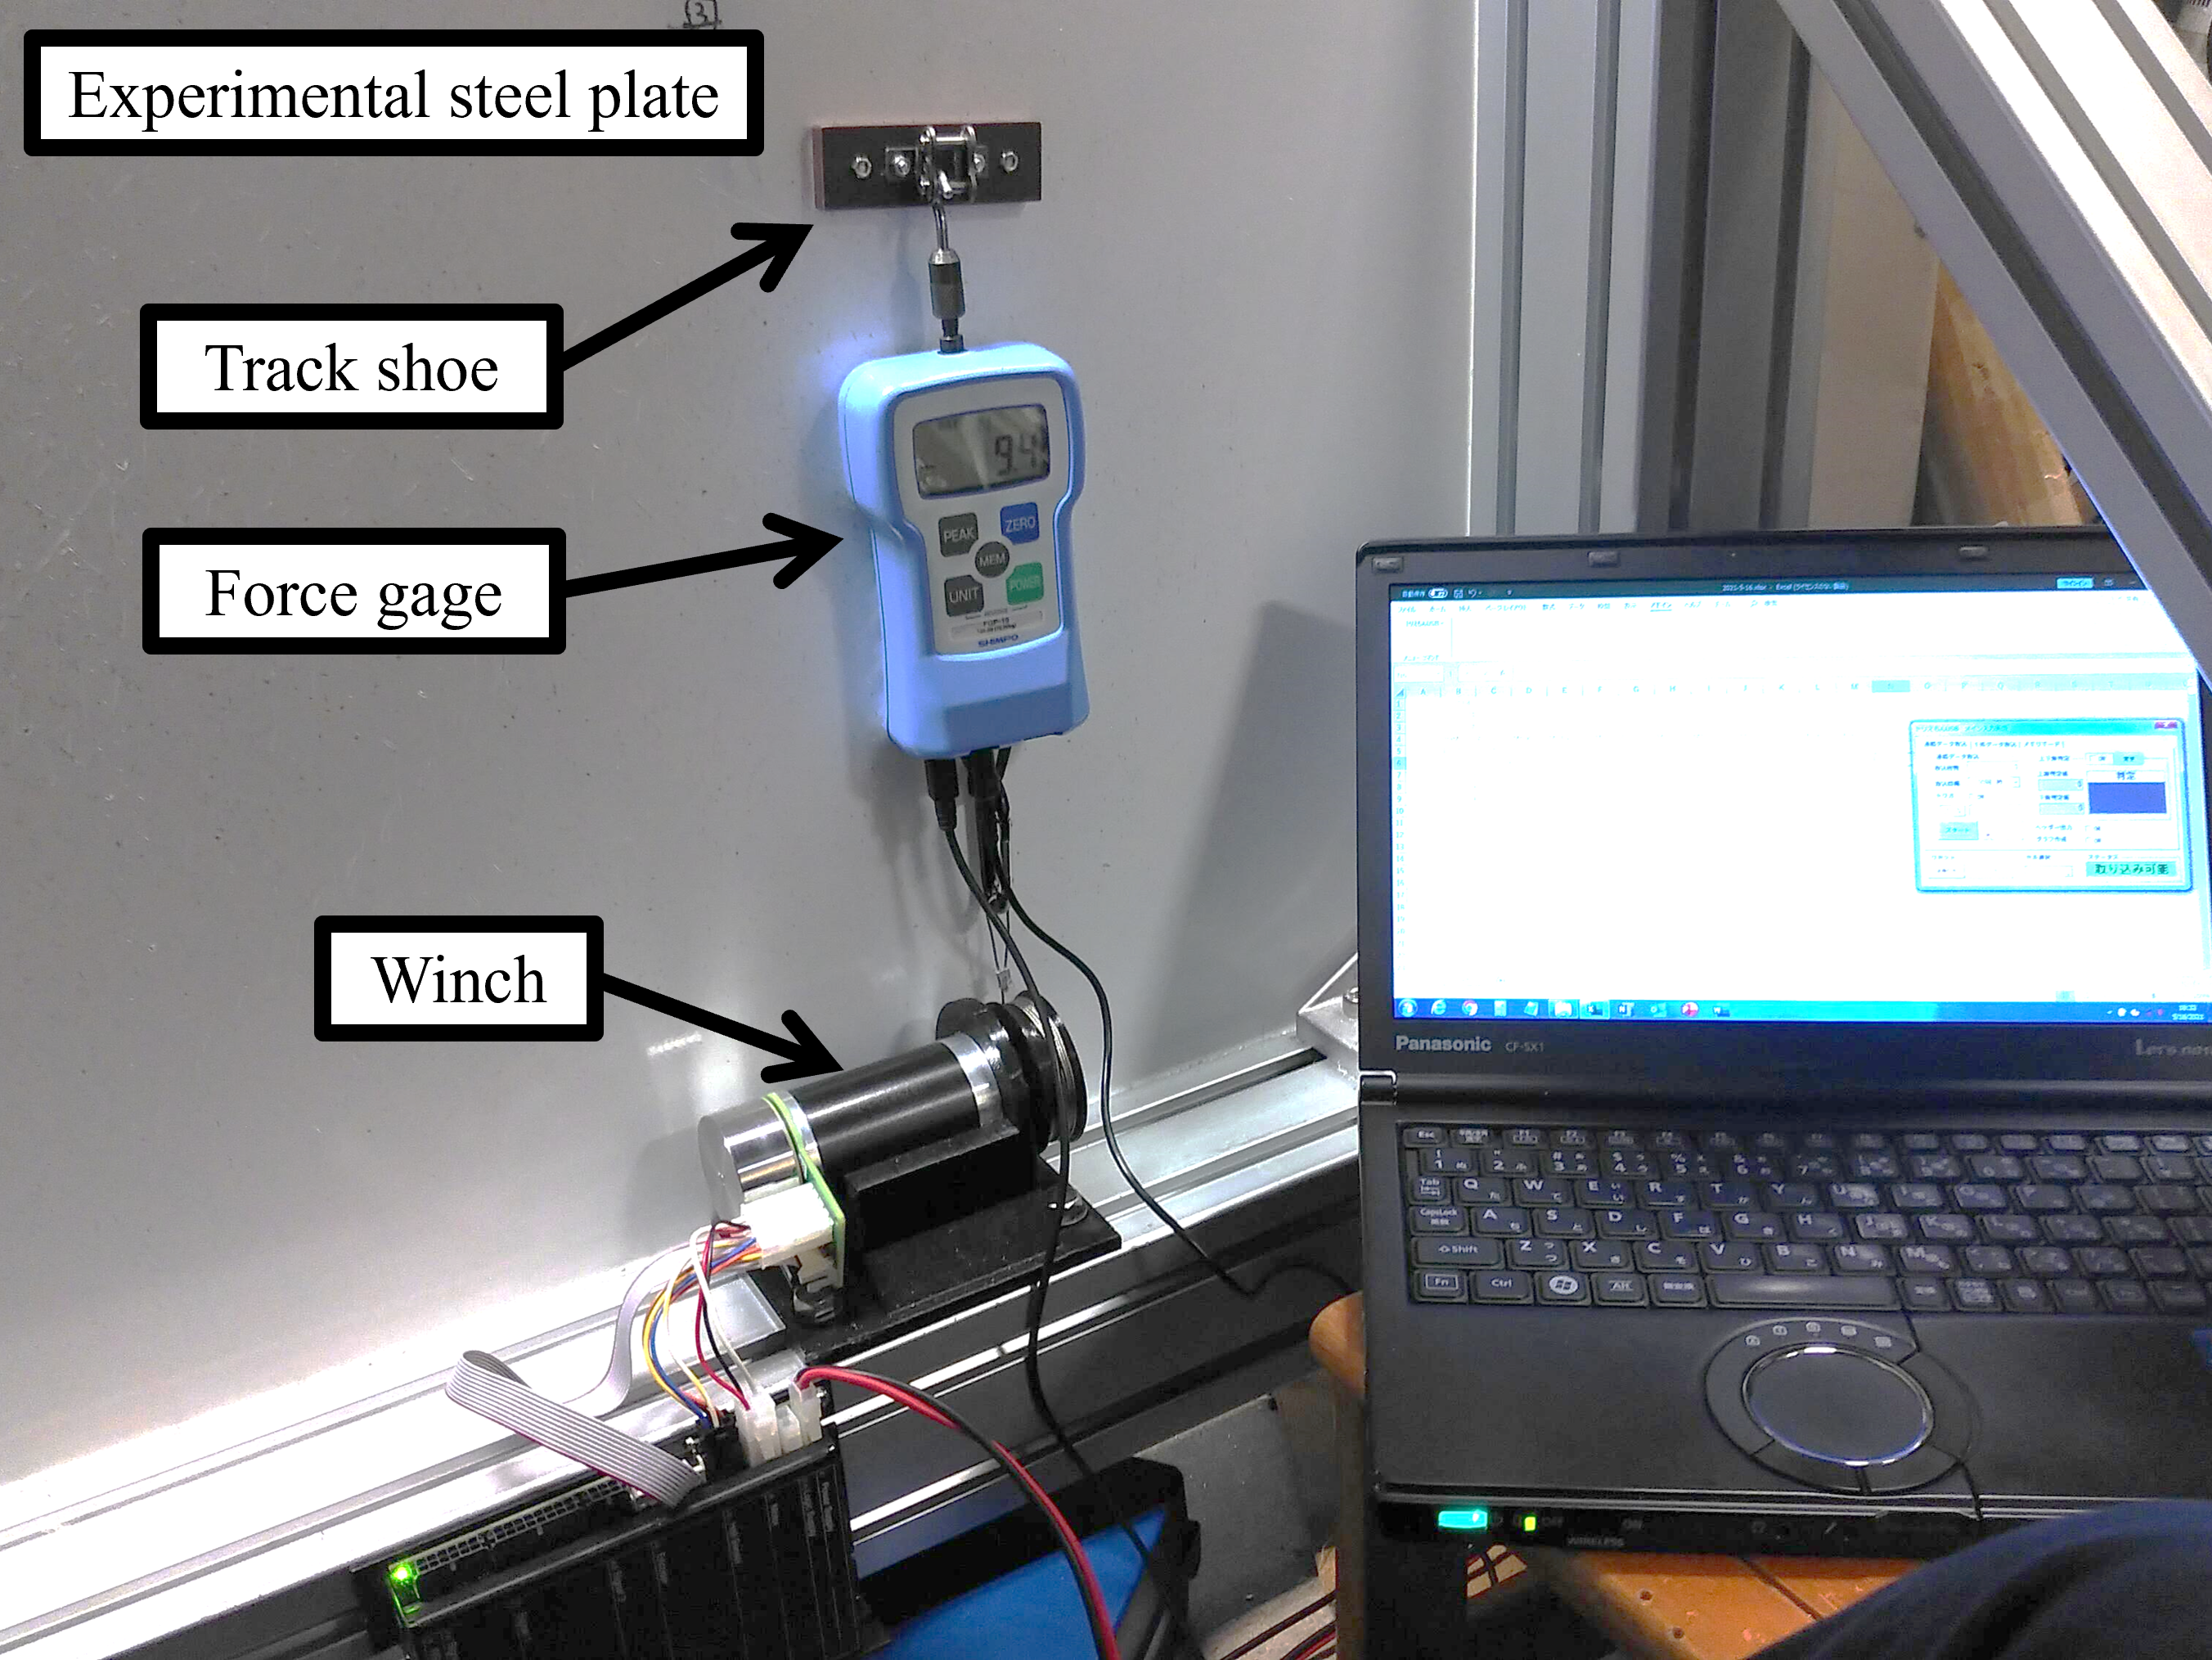
\includegraphics[width=1\textwidth]{full/friction-test.png}
  \caption{Friction testing of track shoe}
  \label{friction-test}
\end{figure}

\subsubsection{静止摩擦力の計測}
ウィンチの引張方向に対し3か所計測ヶ所を設けた. 
3か所についてそれぞれ2回行い計測を行いすべての平均を計算に用いた. 
ウィンチにより1[mm/s]でワイヤーを引っ張り, 動き始めまでにおけるフォースゲージの最大値を計測値とした. 

\newpage
\subsubsection{動摩擦力の計測}
ウィンチを用い静止摩擦力の3か所の計測ヶ所を通過するように50[mm/s]で移動させその間のフォースゲージの連続的な値を取得した. 1[s]~10[s]の平均値を取得した. 計測を3回行いさらにこれで平均を計算に用いた. ABSにおける取得した値のグラフを図\ref{ABS-friction}に示す.

\begin{figure}[H]
  \centering
  \includegraphics[width=1\textwidth]{full/ABS_friction.png}
  \caption{Result of friction test on ABS trackshoe}
  \label{ABS-friction}
\end{figure}

\subsubsection{吸着力の計測方法}
鋼板に対し履板を剥離させる方向にフォースゲージ及びウィンチのワイヤーを配置した. ウィンチを動かし, 履板が鋼板から外れるまでにおけるフォースゲージの最大値を吸着力とした. 静止摩擦力を測ったのと同様の計測箇所で3か所計測を行いその平均値を計算に用いた. 

\begin{figure}[H]
  \centering
  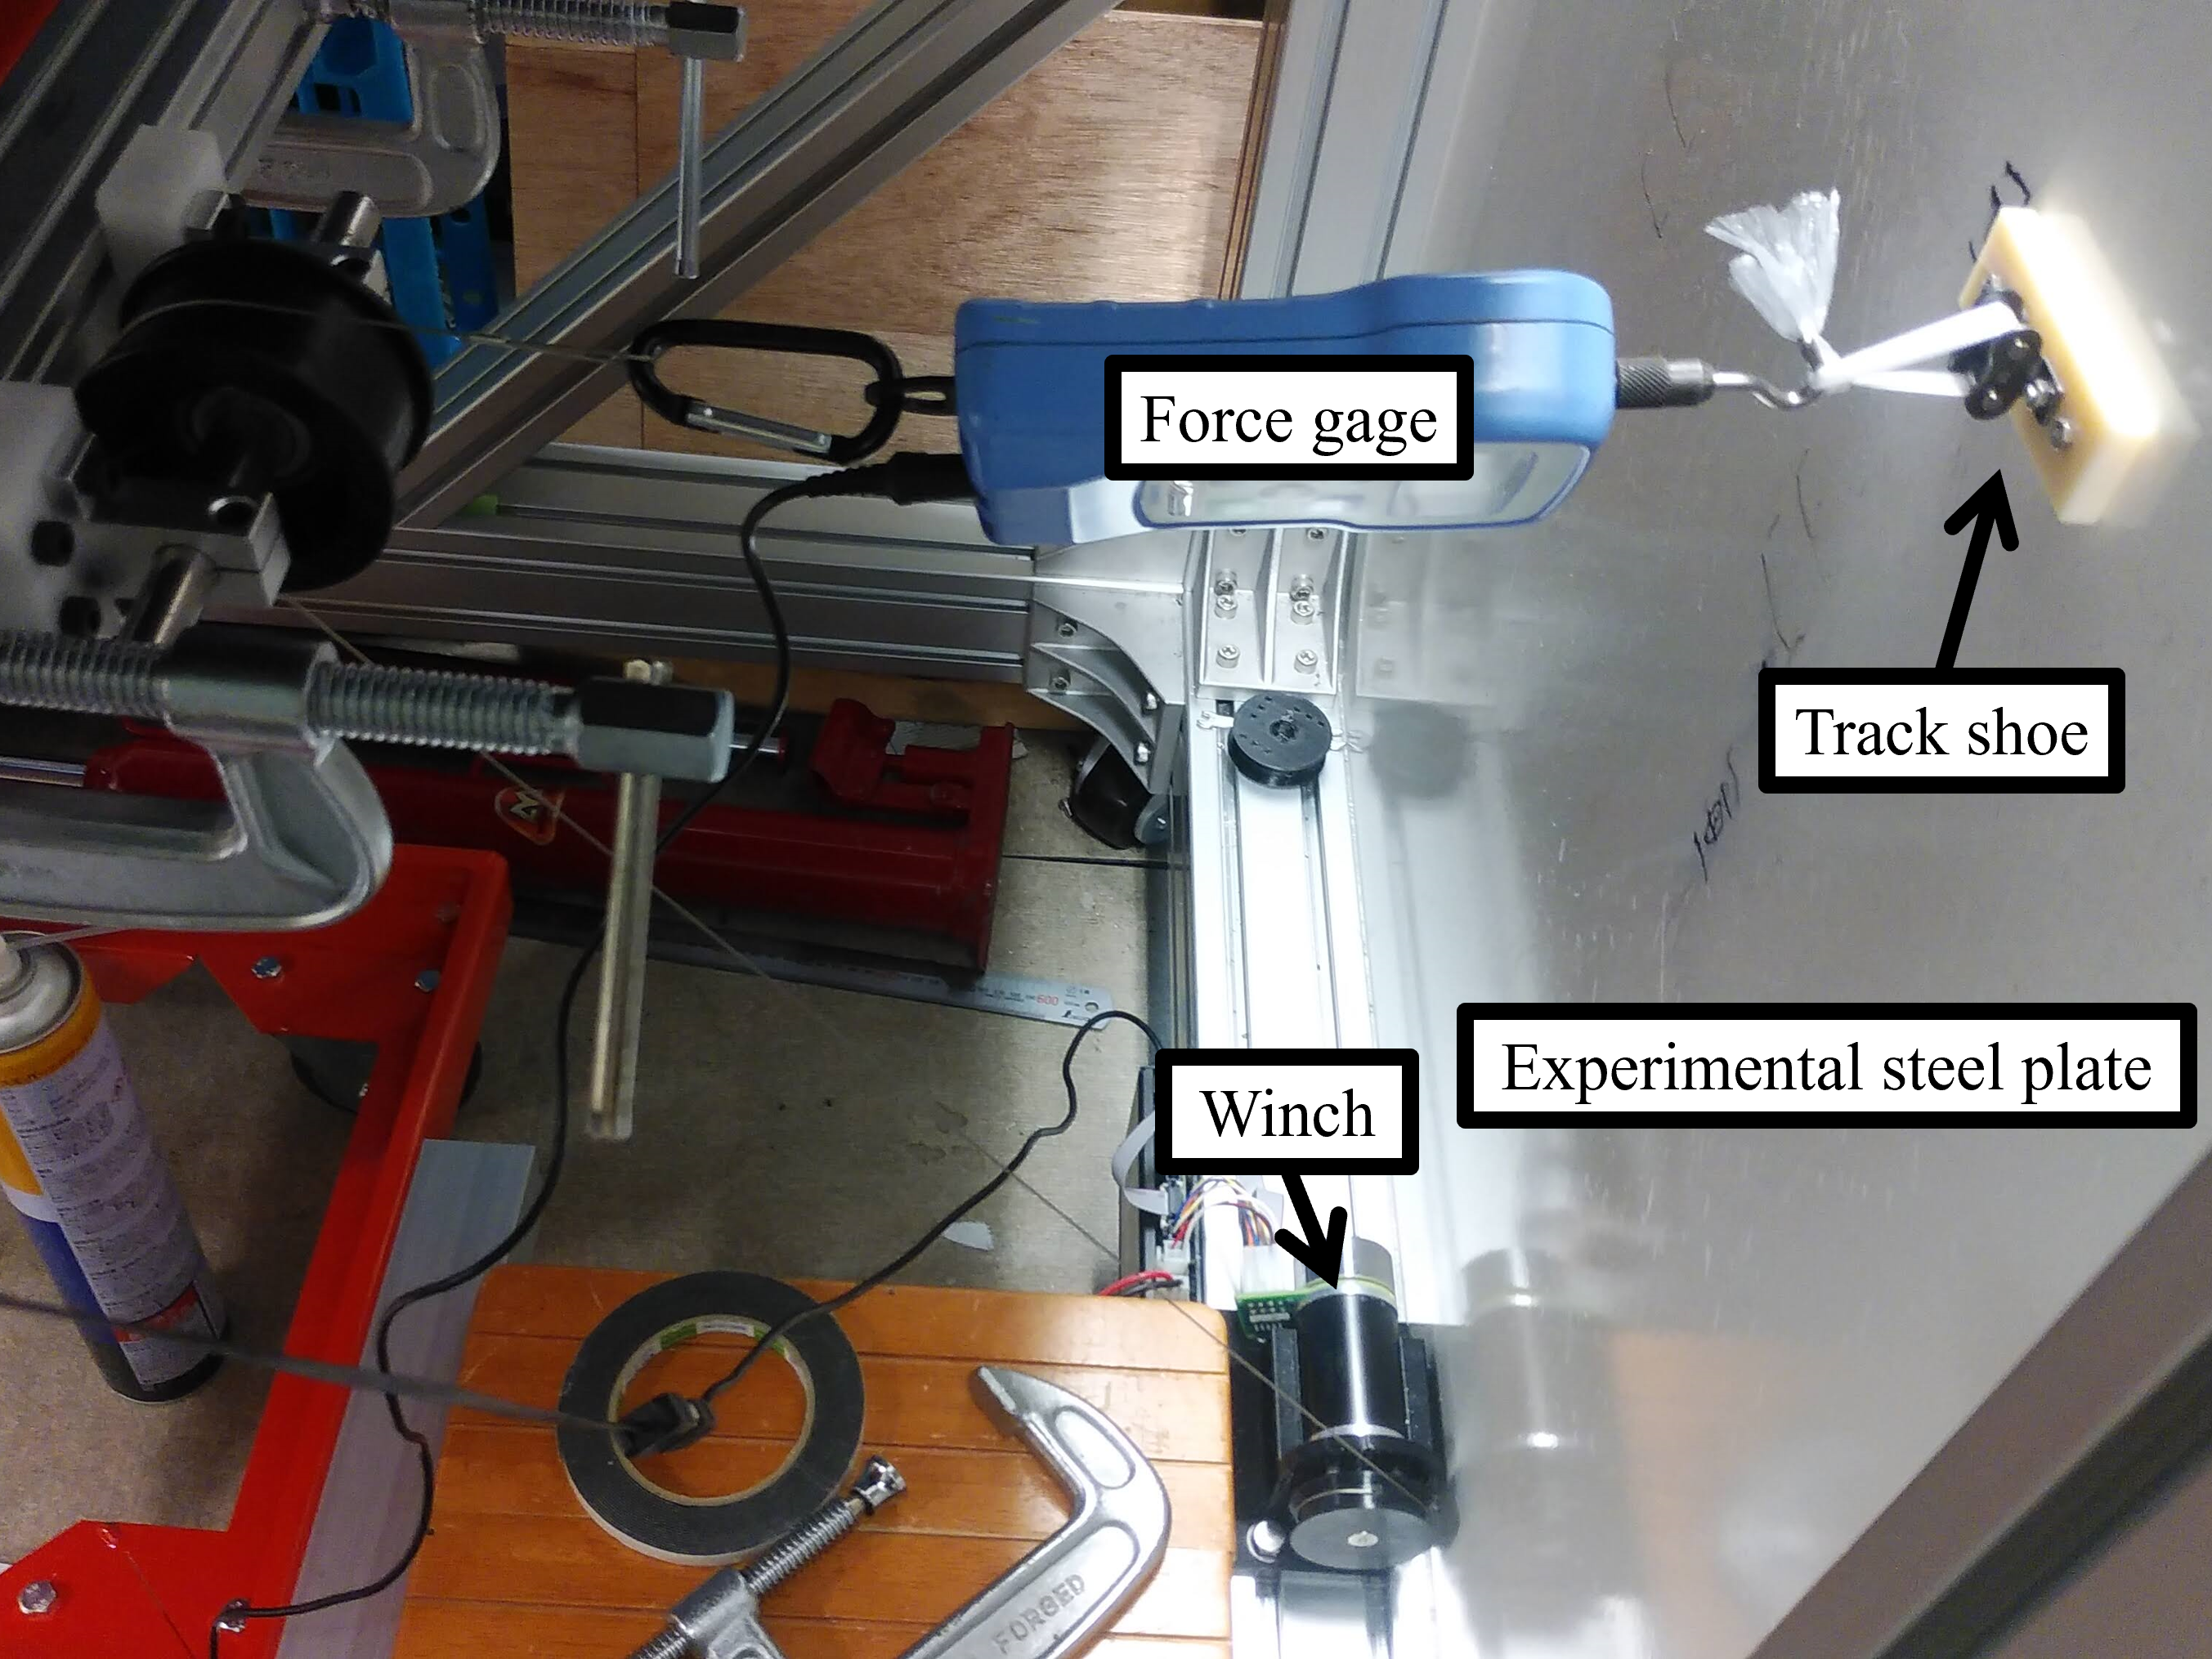
\includegraphics[width=0.7\textwidth]{full/trackshoe_absorb-test.png}
  \caption{Absorb testing of trackshoe}
  \label{absorb-test_pic}
\end{figure}

\subsubsection{結果}

導出した摩擦係数を次のグラフに示す. 
ABSが一番大きい摩擦係数を示したためABSを使用することとした. 

\begin{table}[H]
  \centering
  \caption{Average of adsorption and friction force measurements and coefficient of friction}
  \begin{tabular}{r|ccccc}
                                  & ABS  & PC & MC601ST & MC901 & POM \\ \hline
  Adhesive force {[}N{]}          & 70.3 & 71.4 & 65.5 & 67.4 & 67.4 \\
  Static friction force {[}N{]}   & 42.7 & 37.7 & 37.7 & 40.7 & 28.2 \\
  Dynamic friction force {[}N{]}  & 26.7 & 26.9 & 17.3 & 16.8 & 15.4 \\
  Coefficient of static friction  & 0.61 & 0.53 & 0.57 & 0.60 & 0.42 \\
  Coefficient of Dynamic friction & 0.38 & 0.38 & 0.26 & 0.25 & 0.23  
  \end{tabular}
\end{table}

\begin{figure}[H]
  \centering
  \includegraphics[width=0.9\textwidth]{full/track-shoe_friction.png}
  \caption{Coefficient of friction obtained from test data}
  \label{track-shoe_friction}
\end{figure}

\begin{comment}

\begin{table}[h]
  \centering
  \begin{tabular}{r|cc}
  材料     & 静止摩擦係数 & 動摩擦係数 \\ \hline
  POM     & 0.42   & 0.22  \\
  ABS     & 0.61   & 0.38  \\
  MC901   & 0.60   & 0.25  \\
  MC601ST & 0.57   & 0.26 
  \end{tabular}
\end{table}
  
\end{comment}

\newpage
\subsection{磁石の吸着力計測}
磁石は鋼板との距離に応じて吸着力が減少することが知られている. 吸着力を設計する上で使用する磁石の鋼板との距離と吸着力の関係を明らかにする必要がある. そこで履板に使用する磁石及び, フレーム磁石に使用するヨーク付きの磁石について距離と吸着力を計測した.

\subsubsection{磁石の吸着力計測装置}
磁石の吸着力の計測には米田研究室で製作された装置(図\ref{mesure})を用いた.
この装置は鋼板の上にギアドモータとリードねじによる直動機構が取り付けてある. 
これにロードセルとレーザ変位センサ, 計測対象の磁石を取り付けることにより, 磁石の鋼板との距離と吸着力を同時に計測しその関係を調べることができる.

\begin{figure}[H]
  \centering
  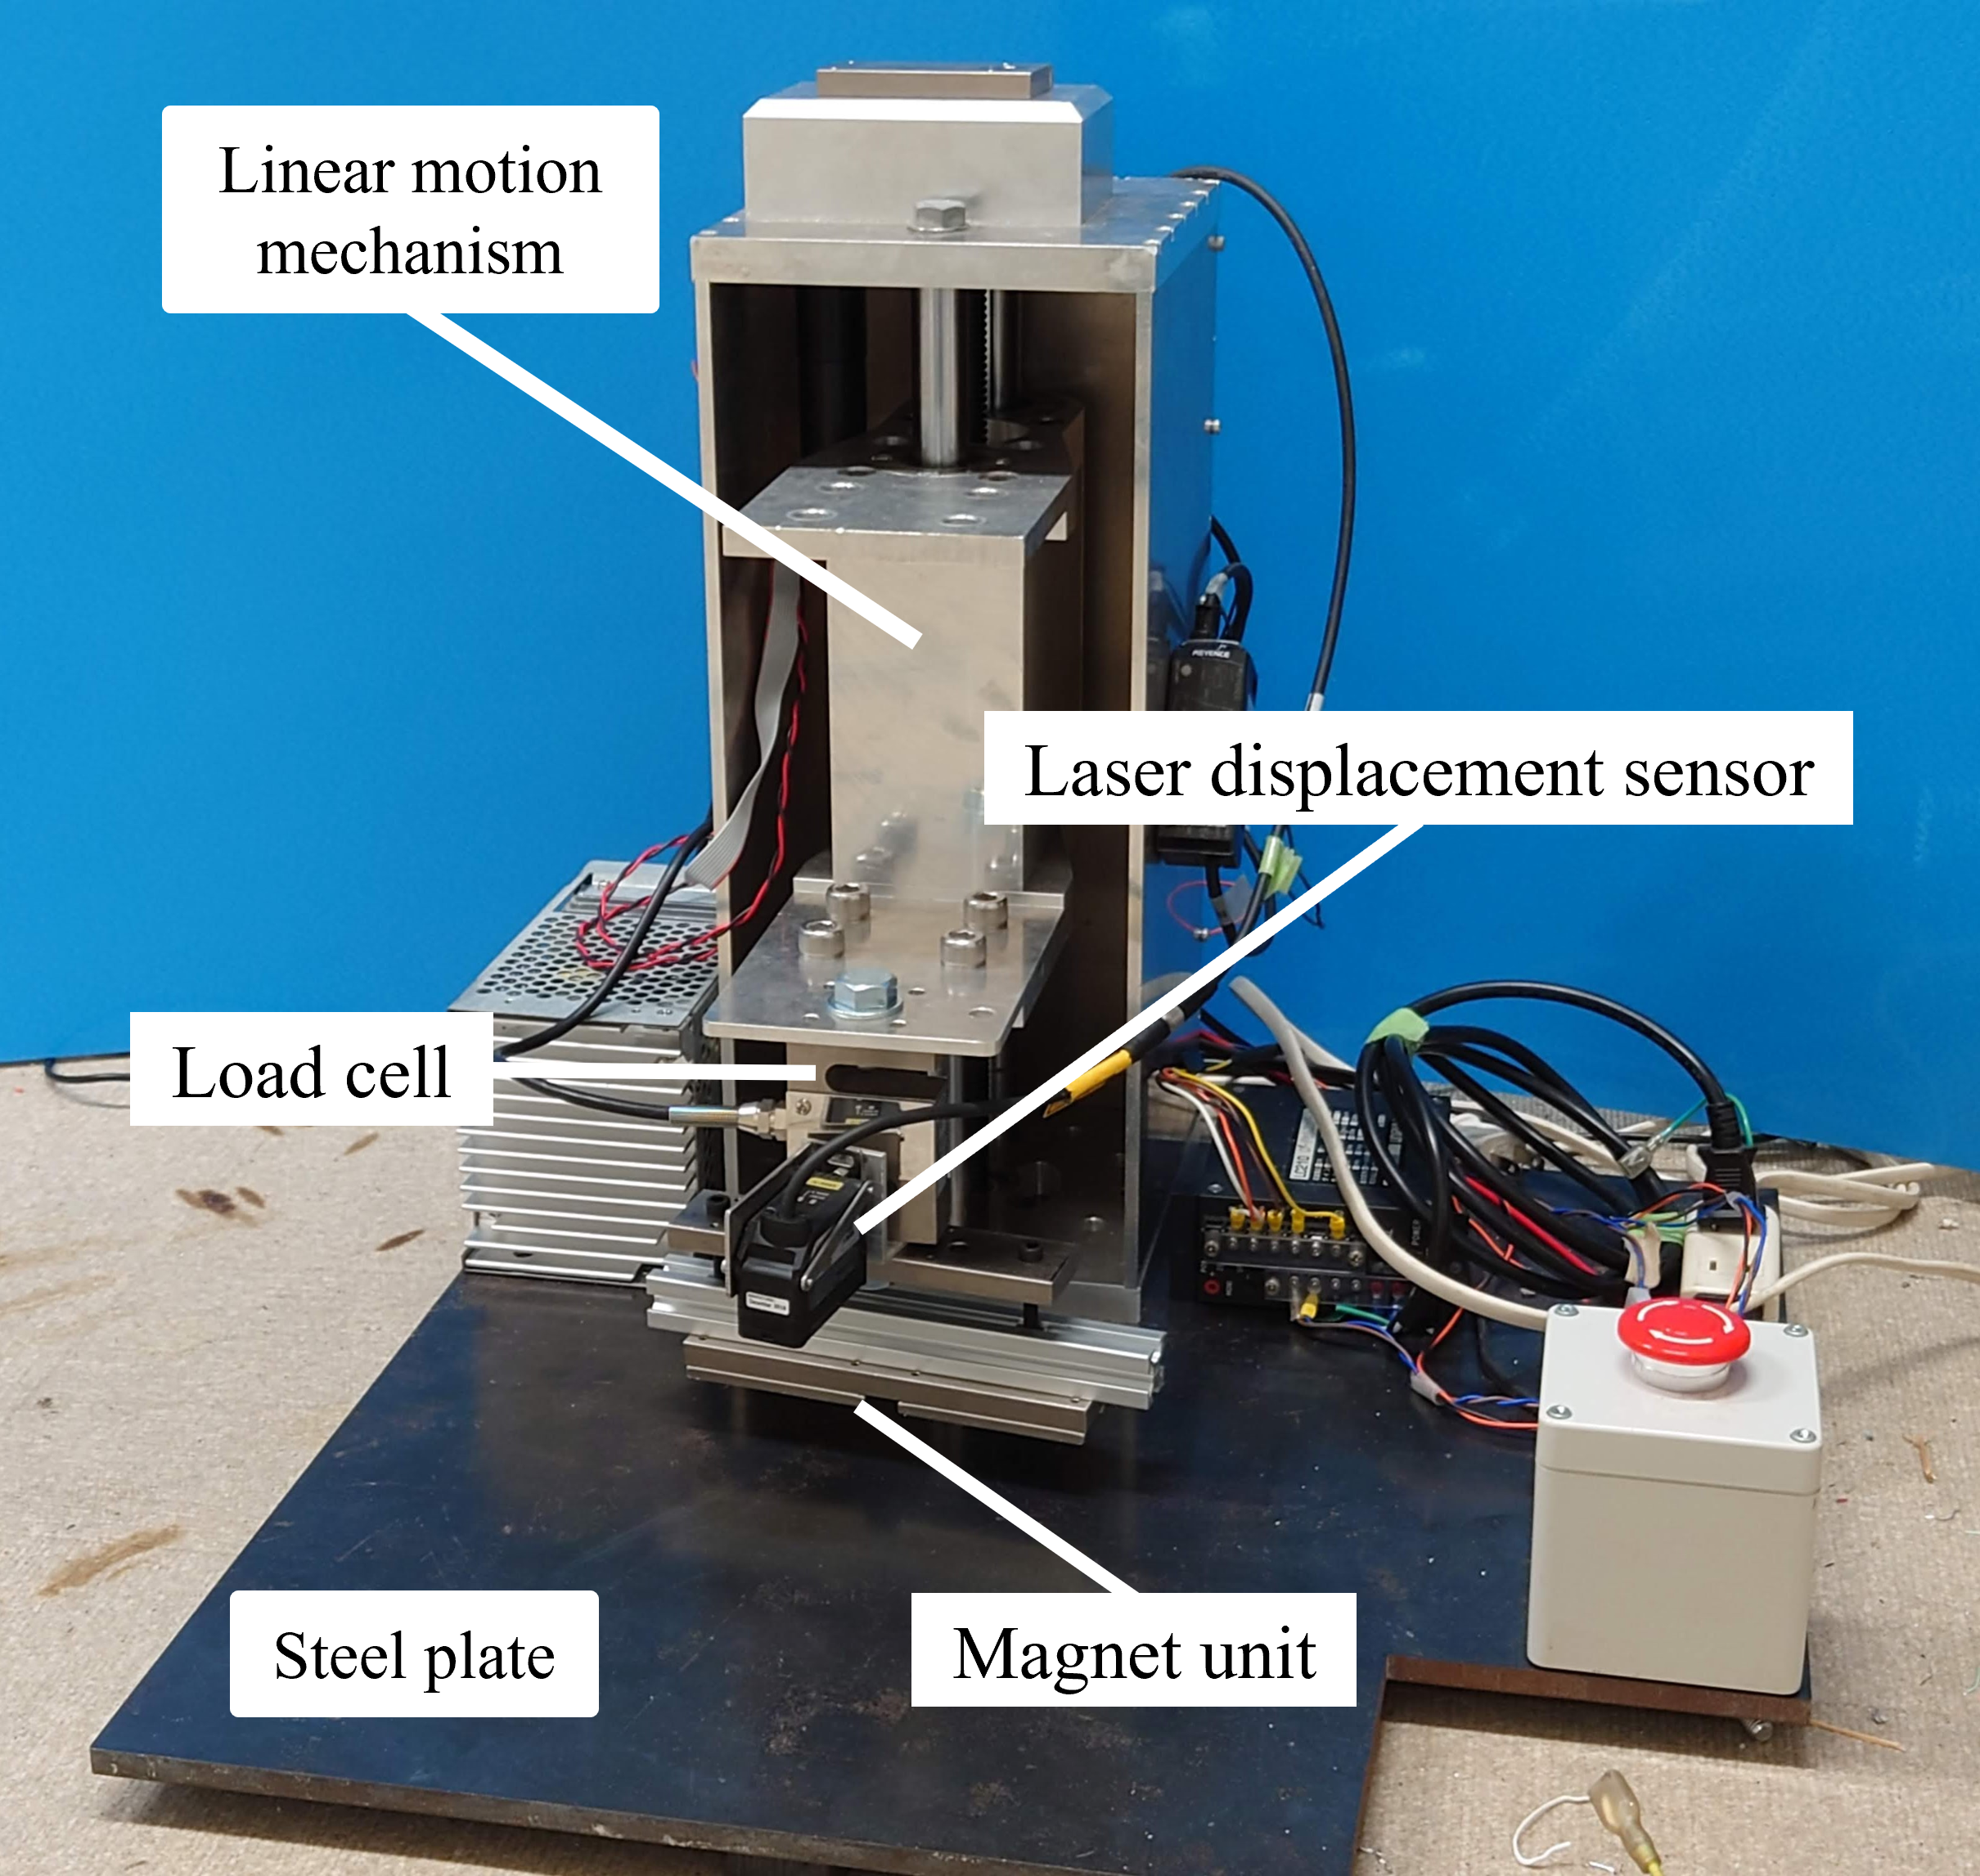
\includegraphics[width=0.9\textwidth]{full/magnet_mesure.png}
  \caption{Machine for measuring the magnetic adhesion force}
  \label{mesure}
\end{figure}

\begin{table}[h]
  \centering
  \caption{Sensor details of the measuring machine}
  \begin{tabular}{ccc}
    Manufacturer & Product name & Model \\ \hline
    Pushton & Load cell & PSD-S1 \\
    KEYENCE & CMOS laser application sensor head & IL-S065 \\ 
    KEYENCE & CMOS laser application Amplifier unit & IL-1000 \\ 
  \end{tabular}
  \label{absorb-machine}
\end{table}

\newpage

\subsubsection{履帯磁石の吸着力試験}
\label{absorb-test}
履帯磁石は履帯に使用するチェーンのピッチや履板の寸法及び取付穴の制約の中でより吸着力の高いものを選定した. 今回はNSC0058(表\ref{magnet-spec},\cite{magfine67})を採用した. 履板磁石に使用する磁石について先述の装置を用いて距離と吸着力の関係を求めた. グラフを下記に示す. 吸着力が表\ref{magnet-spec}のカタログ値を下回るのはカタログ値が純度の高い鉄との吸着力であるのに対し, 今回の吸着対象は炭素鋼であるからだと考えられる.

塗膜厚0.7[mm]と履板接地面と磁石の距離0.3[mm]を足した鋼板とのギャップ1[mm]のNとSの平均値は64.06[N]となった.


\begin{table}[H]
  \centering
  \caption{Specification of magnets (Catalog value)}
  \label{magnet-spec}
  \begin{tabular}{r|cc}
                                  & NSC0058       & NSC0075       \\ \hline
  Distributor                     & \multicolumn{2}{c}{Magfine}   \\
  Material                        & \multicolumn{2}{c}{Neodymium 35} \\
  Size                            & 67x10x5[mm]   & 60x10x5[mm]   \\
  Adhesion force                  & 195.0[N]      & 168.6[N]      \\
  Upper working temperature limit & 70[\si{\degreeCelsius}]        & 75[\si{\degreeCelsius}]
  \end{tabular}
\end{table}


\begin{figure}[H]
  \begin{minipage}{0.5\hsize}
    \centering
    \includegraphics[width=1\textwidth]{full/magnet1_absorb-test.png}
    \caption{N magnet absorb test}
    \label{Nmag}
  \end{minipage}
  \begin{minipage}{0.5\hsize}
    \centering
    \includegraphics[width=1\textwidth]{full/magnet1_absorb-test_S.png}
    \caption{S magnet absorb test}
    \label{Smag}
  \end{minipage}
\end{figure}	


\subsubsection{ヨーク付き磁石の吸着力試験}
一般的に磁石はヨーク(継鉄)を用い吸着面に磁束を集中させることで, 吸着力が高まることが知られている. フレーム磁石の設計にあたり, ヨークの効果を確認する試験を行った. 磁石は当初フレーム磁石への使用を検討していたNSC0075(表\ref{magnet-spec},\cite{magfine60})を用いた. ヨークには厚さ6[mm]のSS400と思われる鋼材を用いた.  
今回使用したロードセルの定格荷重の関係から, t1のアルミ板を用いあらかじめ1[mm]距離を取った状態で行った.

磁石間の距離を増やすことで漏れ磁束が減り, 吸着力が向上すると考え, 磁石間の距離を3通り試した(図\ref{0mm}~\ref{10mm}). 結果, 予想と一致し一番大きい距離の磁石ユニットの吸着力が最も大きくなった(図 \ref{yoke-graph}). ヨークを用いることで用いない磁石と比較し3倍以上の吸着力を確認することができた.

\begin{figure}[H]
  \begin{minipage}{0.5\hsize}
    \centering
    \includegraphics[width=1\textwidth]{full/yoke0.png}
    \caption{Magnet unit with yoke with 0[mm] magnet spacing}
    \label{0mm}
  \end{minipage}
  \begin{minipage}{0.5\hsize}
    \centering
    \includegraphics[width=1\textwidth]{full/yoke5.png}
    \caption{Magnet unit with yoke with 5[mm] magnet spacing}
    \label{5mm}
  \end{minipage}
\end{figure}	

\begin{figure}[H]
  \centering
  \includegraphics[width=0.5\textwidth]{full/yoke10.png}
  \caption{Magnet unit with yoke with 10[mm] magnet spacing}
  \label{10mm}
\end{figure}

\begin{figure}[H]
  \centering
  \includegraphics[width=1\textwidth]{full/yoke_graph.png}
  \caption{Adsorption force test results of magnet with yoke}
  \label{yoke-graph}
\end{figure}

\newpage

実際の機体では使用する磁石と寸法を変更することとしたため, 再度吸着力の計測を行った. 磁石はNSC0058に変更し, ヨークの厚さを9[mm], 磁石の間隔を12[mm]とした. また, 材料はSS400とした. 

塗膜厚0.7mmと壁面とフレーム磁石のギャップを1[mm]とした場合, これを足した鋼板とのギャップ1.7[mm]の時の吸着力は, 592.18[N]となった. また, これを4で除した磁石1個当たりの吸着力は148.04[N]となった.

\begin{figure}[H]
  \centering
  \includegraphics[width=0.7\textwidth]{full/yoke_graph_full.png}
  \caption{Adhesive force test results of a magnet with a yoke similar to that used in a full scale robot}
  \label{yoke-graph-full}
\end{figure}

\newpage

\subsection{必要な吸着力の設計}

下記に設計に用いた吸着力の計算について述べる. 必要な吸着力は履板磁石とフレーム磁石の合計となる. 履板磁石の個数は機体のサイズの制約により決まる. そのため, 必要な吸着力から履板磁石による吸着力を引いた値, すなわちフレーム磁石が担う必要がある吸着力を求めた. これをフレーム磁石1個当たりの吸着力で除することにより, 必要なフレーム磁石の個数を求め設計の参考とした. また, 塗膜厚は塗り重ねのない場合の最大値とされる0.7[mm]を想定した.



\vspace{6mm}\noindent\textgt{必要な吸着力の導出}\\
\vspace{-4mm}
\begin{equation}
  \label{eq_of_absorb}
  \frac{目標機体重量\:50[\mathrm{kg}] \times 重力加速度\:9.8[\mathrm{m/s^2}] \times 必要な重量と動摩擦力の比\:3.5}{動摩擦係数\:0.38} \approx 4513[\mathrm{N}]
\end{equation}

\vspace{6mm}\noindent\textgt{履板磁石による吸着力の導出}\\
1/2スケール機体の検証においてクローラユニット動摩擦力は履板1つの動摩擦力の個数倍に対し約0.79の割合であったため(表\ref{friction})今回求めるのは吸着力だが, 動摩擦力に作用する吸着力と考え, 今回の計算ではこれを合計摩擦力係数として計算に含めた. 
また履板一枚の吸着力については\ref{absorb-test}の吸着力試験における塗膜厚0.7[mm]と履板接地面と磁石の距離0.3[mm]を足した鋼板とのギャップ1[mm]のNとSの平均値を用いた. 

\begin{equation}
  履板一枚の吸着力\:64.06[\mathrm{N}] \times 設置履板枚数\:34 \times 合計摩擦力係数\:0.79 \approx 1721[\mathrm{N}]
\end{equation}


\vspace{6mm}\noindent\textgt{フレーム磁石の吸着力の導出}\\
\vspace{-1mm}
\begin{equation}
  必要な吸着力\:4513[\mathrm{N}] - 履板磁石による吸着力\:1721[\mathrm{N}] = 2792[\mathrm{N}]
\end{equation}
	
\vspace{6mm}\noindent\textgt{必要なフレーム磁石の個数の導出}\\
塗膜厚0.7mmと壁面とフレーム磁石のギャップを1[mm]とし, これを足した鋼板とのギャップ1.7[mm]の時のヨーク付き磁石の吸着力試験の値を用いた. 

\begin{equation}
  必要なフレーム磁石の吸着力\:2792[\mathrm{N}] \div フレーム磁石1個当たりの吸着力\:148.04 \approx 19[個]
\end{equation}

\vspace{4mm}

以上の計算により最低限必要なフレーム磁石の個数は約19個であると予想できた. 設計においては摩擦係数の低下や重量の増加なども考慮し40個のフレーム磁石を使用することとした.
よって必要な吸着力に対し$\frac{40}{19}\approx 2.12$倍の余裕を見込むことができると考えた. 上述の計算ではフレーム磁石と壁面のギャップを塗装の凸凹等に対し大きな余裕を持った値を設定しているが, これをより小さく設定することでさらに大きい吸着力を得ることができる. 

\newpage

\subsection{クローラユニットの動摩擦力の計測}
\label{test_friction_crawler}
クローラユニットの動摩擦力が設計通りか確認するために, クローラユニット単体での動摩擦試験を行った. 実験用鋼板を固定しているフレームに引張方向で拘束させたフォースゲージをクローラユニットとフォースゲージをワイヤーで接続し, クローラを駆動させ, 一定時間のフォースゲージの値を読み取った(図\ref{crawler_friction-test}).

\begin{figure}[H]
  \centering
  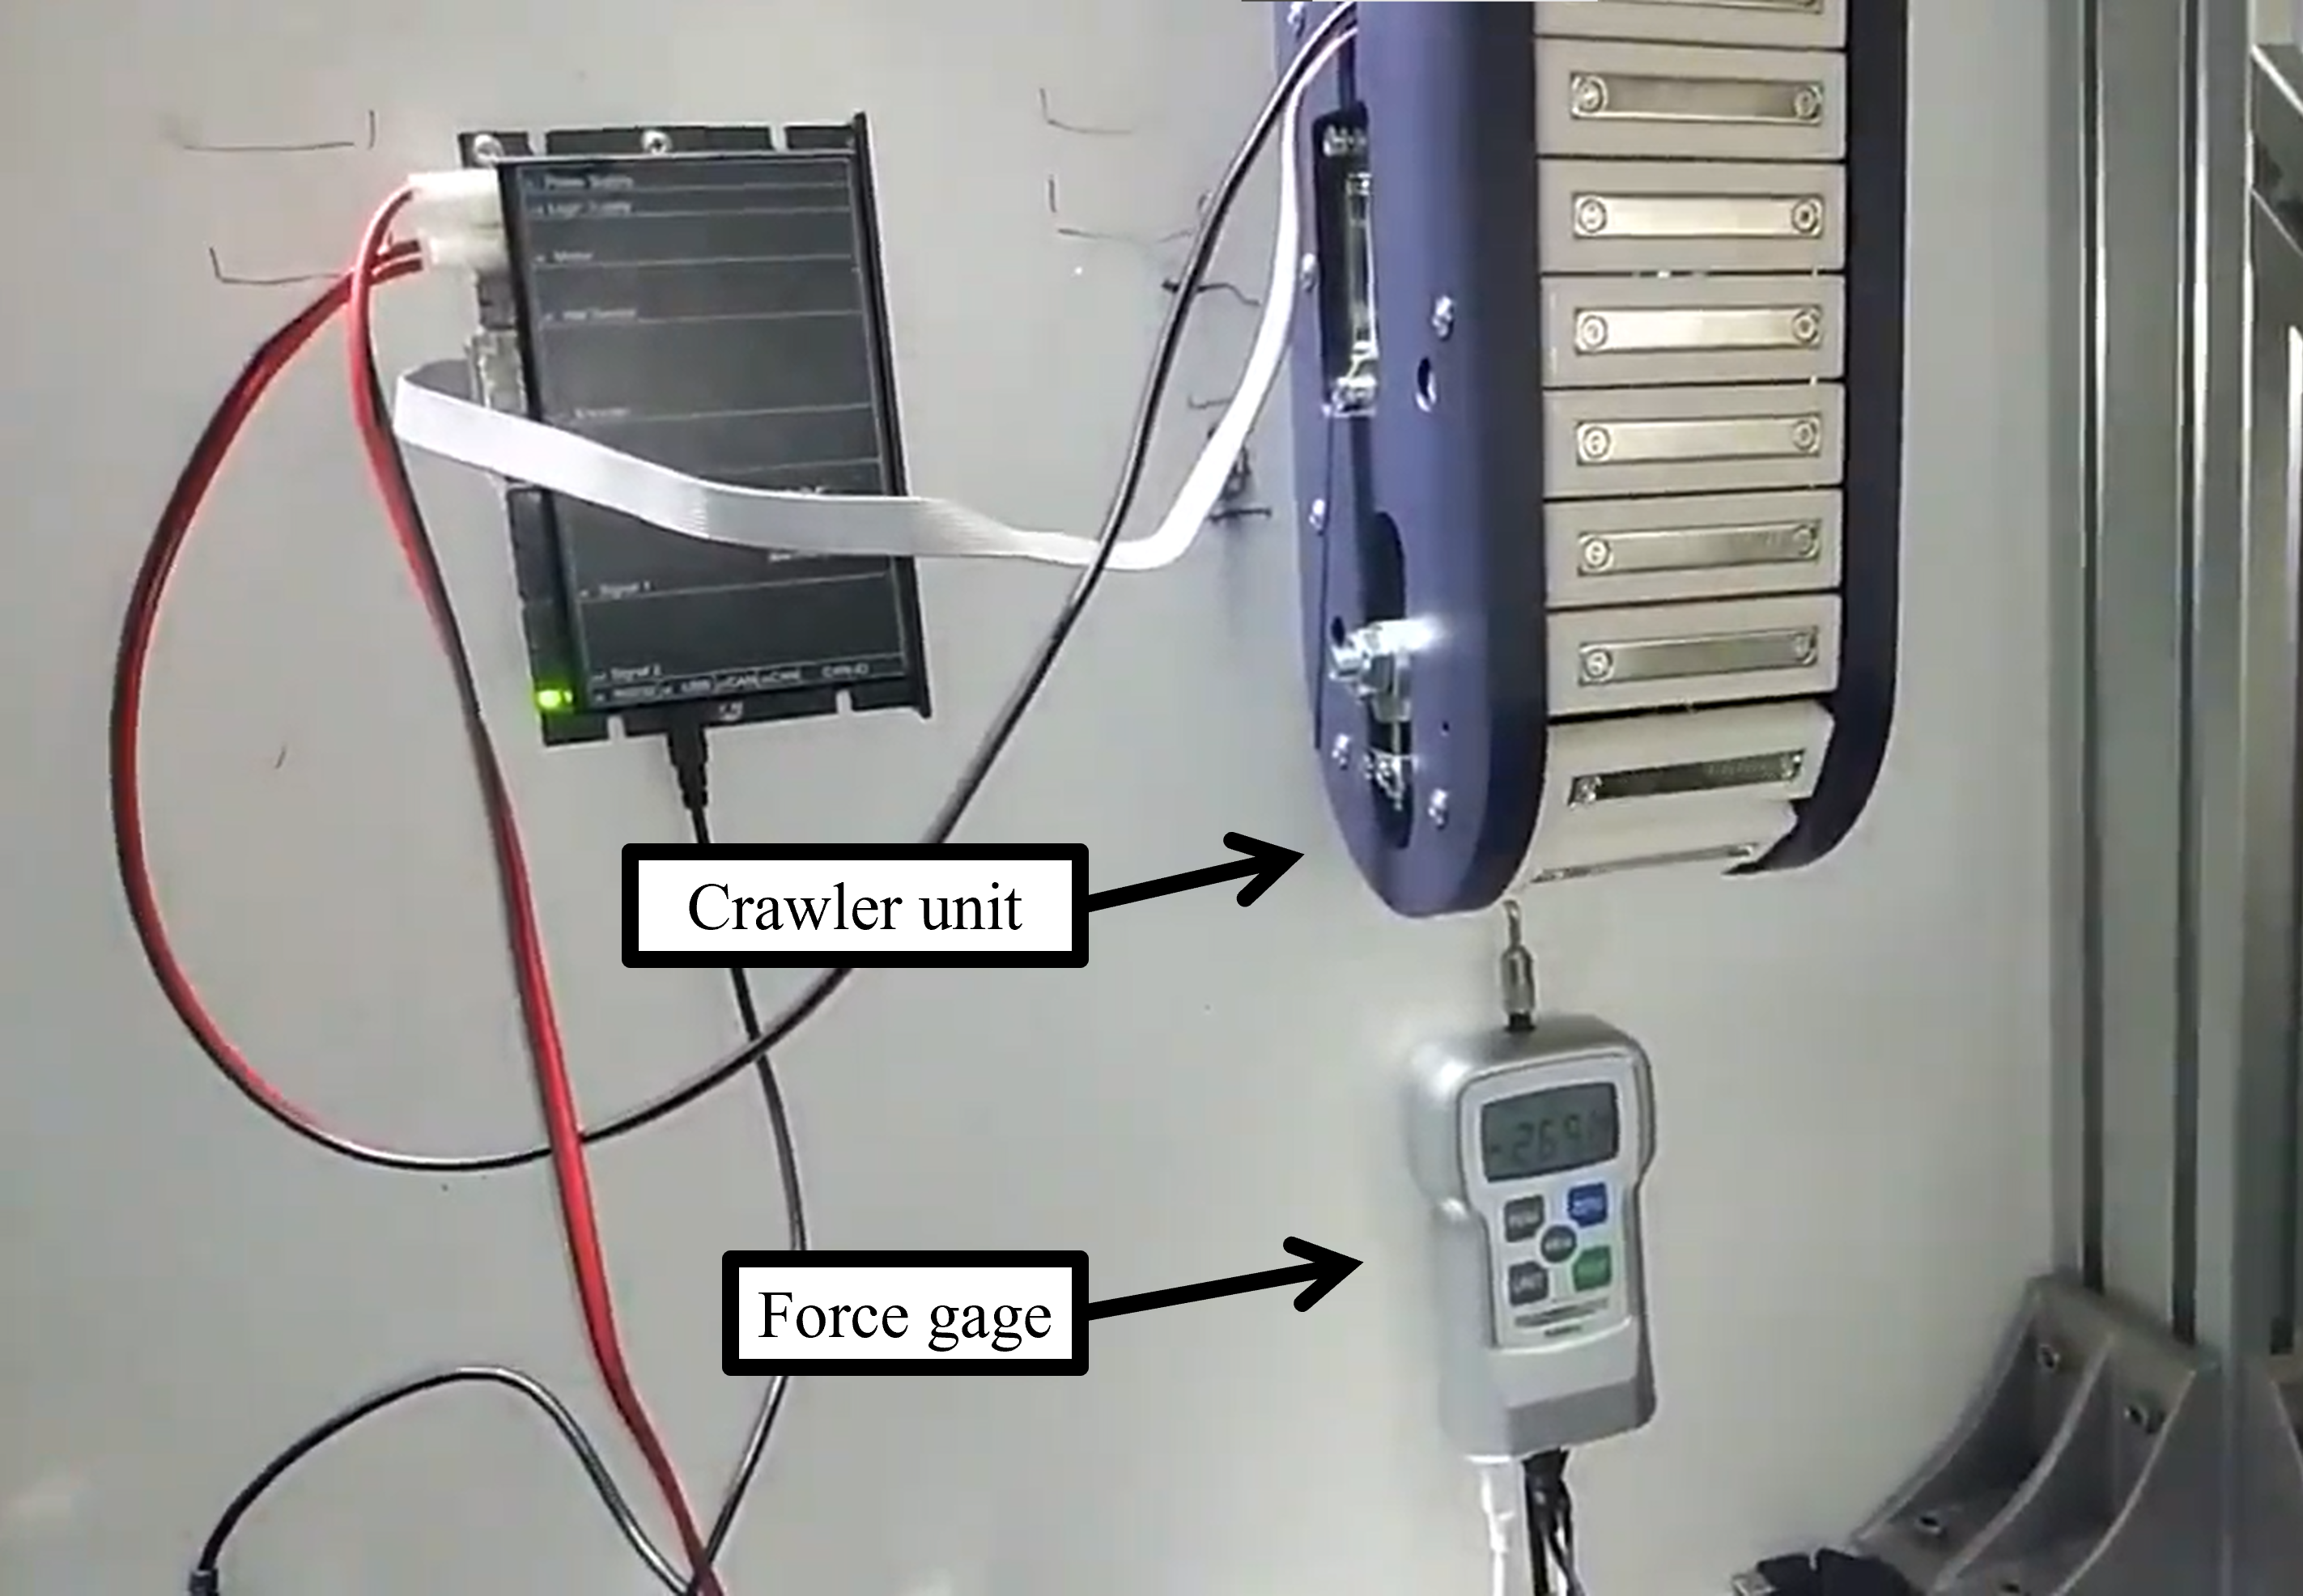
\includegraphics[width=0.6\textwidth]{full/Crawler_friction-test.png}
  \caption{Friction testing of crawler unit}
  \label{crawler_friction-test}
\end{figure}

結果のグラフを以下に示す. 今回の計測では, 参考のため速度を変えて計測も行った.
基準としている速度50[mm/s]における10~25[s]の平均は410[N]であった.
これを設計値と比較する.
今回計測を行った個所の塗膜厚の平均は0.33[mm]であり, 機体の履板の接地面と磁石の距離が0.3[mm]であるため, \ref{absorb-test}の試験より, 0.63[mm]の吸着力の平均値である79.60[N]を計算に使用した.
式\ref{eq_of_crawler-friction}により求められる吸着力の設計値は計測値とおおむね一致しており設計通りの動摩擦力が得られていることが確認できた. また, 速度と動摩擦係数に相関性があることが確認できた.

\begin{equation}
  履板磁石の吸着力\:79.60[N] \times 履板設置枚数\:17 \times 合計吸着力係数\:0.79 \times 動摩擦係数\:0.38 \approx 406[N]
  \label{eq_of_crawler-friction}
\end{equation}

\begin{figure}[H]
  \centering
  \includegraphics[width=0.8\textwidth]{full/crawler_friction.png}
  \caption{Friction of crawler unit}
  \label{friction crawler}
\end{figure}


\subsection{機体全体の動摩擦力の評価}
\ref{select}~\ref{test_friction_crawler}で得られたデータをもとに, 機体全体の動摩擦力を評価した. 以下に動摩擦係数$\mu' = 0.38$ 塗膜厚$t=0.5$の時のフレーム磁石と壁面の距離と機体の動摩擦力の関係のグラフを以下に示す. 青と紫で塗りつぶした部分がそれぞれ履帯磁石とフレーム磁石により得られる動摩擦力を示す. 今回の条件の場合, フレーム磁石と壁面の距離を約3.3[mm]に調整することで滑り落ちずに旋回するのに必要な重量の3.5倍の動摩擦力を得られることが確認できる. 

\begin{figure}[H]
  \centering
  \includegraphics[width=1\textwidth]{eva/ajst1.png}
  \caption{Relations of dynamic friction force and distance between frame magnet and wall surface / Frictional force by frame magnet and body magnet}
  \label{ajst1}
\end{figure}

\newpage

次に, 異なる塗膜厚や動摩擦係数の時の動摩擦力を追加したグラフを以下に示す. 運用を想定している壁面において最も厳しいと考えられる条件である$\mu'=0.24$, $t=0.7$の時も青矢印が示すようにフレーム磁石の調整により必要な動摩擦力を得られることが確認できる. また, 逆に塗装剥離後を想定した$\mu'=0.5$, $t=0$の時にも対応できることも確認できた. 

\begin{figure}[H]
  \centering
  \includegraphics[width=1\textwidth]{eva/ajst2.png}
  \caption{Relations of dynamic friction force and distance between frame magnet and wall surface / Image of adjusting the distance between the frame magnet and the wall surface}
  \label{}
\end{figure}

%\section{駆動部の設計}
%\subsection{モータ及び減速比の設計}

\newpage

\section{レール及び履板の設計}
1/2スケール試作機では, 第\ref{本論}章\ref{displacement}で述べたように履板が履板が壁面に張り付く際, 振動が起きるという問題があった. この問題を解決するために, レール及び履板の形状を工夫した. 

\subsection{レールの形状}
図\ref{normal_crawler},\ref{lifted_crawler}に2種類のクローラの端部の模式図を示す. 本機体においては一点鎖線がレールの中心に該当する. 1/2スケール機体においては図\ref{normal_crawler}のように2つの半円弧を2本の接線で繋ぐ形状である. これに対しフルスケール機体では, 図\ref{lifted_crawler}のように片側に2つの円弧を用い底面(壁面に接触する面)をスプロケット中心軸の円弧の接線から下にオフセットすることでチェーンとスプロケットの接触による振動の影響の軽減を目指した.

\begin{figure}[H]
  \begin{minipage}{0.5\hsize}
    \centering
    \includegraphics[width=1\textwidth]{full/rail_image_0.png}
    \caption{Noamal crawler}
    \label{normal_crawler}
  \end{minipage}
  \begin{minipage}{0.5\hsize}
    \centering
    \includegraphics[width=1\textwidth]{full/rail_image_1.png}
    \caption{Lifted crawler}
    \label{lifted_crawler}
  \end{minipage}
\end{figure}	

次に実際のレールの円弧部の寸法図を示す. 上部のレールは走行の機能とは関係がなく, 余分な摩擦を減らしチェーンの伸びを吸収できるようにするため遊びを大きくとった. 先行研究\cite{magnetic-clawlar}~\cite{magnetic-clawlar3}では, レールは走行部のみとなっているが本研究においては, レールの出口と入り口において引っかかりや異物の侵入などの問題を防ぐため, また作業者の服などの巻き込みを防ぐために全周をレールとする設計とした.

\begin{figure}[H]
  \centering
  \includegraphics[width=0.4\textwidth]{full/rail_plan.png}
  \caption{Arc section of rail}
  \label{arc}
\end{figure}

\newpage

\subsection{履板の形状}
第\ref{本論}章\ref{displacement}で述べた振動を軽減するために, 履板の角にフィレットを設けた.
これにより, レールとピンに遊びがないと仮定した場合, 履板が壁面に張り付く際の履板の角がすでに壁面に接触している履帯よりも壁面方向に飛び出る問題を解消した. \textgt{付録B}に履板の外注図面を掲載した.

\begin{figure}[H]
  \begin{minipage}{0.5\hsize}
    \centering
    \includegraphics[width=1\textwidth]{full/trackshoe_kado.png}
    \caption{Non fillet track}
    \label{non-fillet}
  \end{minipage}
  \begin{minipage}{0.5\hsize}
    \centering
    \includegraphics[width=1\textwidth]{full/trackshoe_fillet.png}
    \caption{Fillet track}
    \label{yes-fillet}
  \end{minipage}
\end{figure}	

さらに, 振動のもう一つの原因であるレールの遊びを少なくした. 1/2スケール機体との寸法の比較を以下の表に示す.

\begin{table}[H]
  \centering
  \caption{Pin and rail comparison between 1/2 scale and full scale robot}
  \begin{tabular}{r|cc}
                       & Half scale prototype & Full scale \\ \hline
  Pin diameter         & 1.5[mm]              & 3[mm]      \\
  Rail width           & 2[mm]                & 3.4[mm]    \\
  Pin play relative to rail & 0.5[mm]         & 0.4[mm]    \\
  Pin dia / Rail width & 0.75                 & 0.88        
  \end{tabular}
\end{table}

\newpage

\section{IHヘッドと壁面の変位の計測}
第\ref{本論}章\ref{displacement}と同様にロボットを走行させた際のIHヘッドと壁面の変位を計測した. フルスケール機体においては, IHヘッドにレーザ変位センサを取り付けることで実際と近い条件で計測を行った. 結果を\ref{dis_full}に示す. 1/2スケール試作機と変位の最大値比較すると, フレーム磁石使用時の変位は増えているがフレーム磁石未使用時の変位は大幅に減少していることが分かる. 前節のレールや履板の設計の工夫によるものと考えられる. これにより, 本体磁石の有無により最大の変位の差が大幅に小さくなり, フレーム磁石と壁面の距離の調整による影響を受けにくいことが確認できた.

\begin{figure}[H]
  \centering
  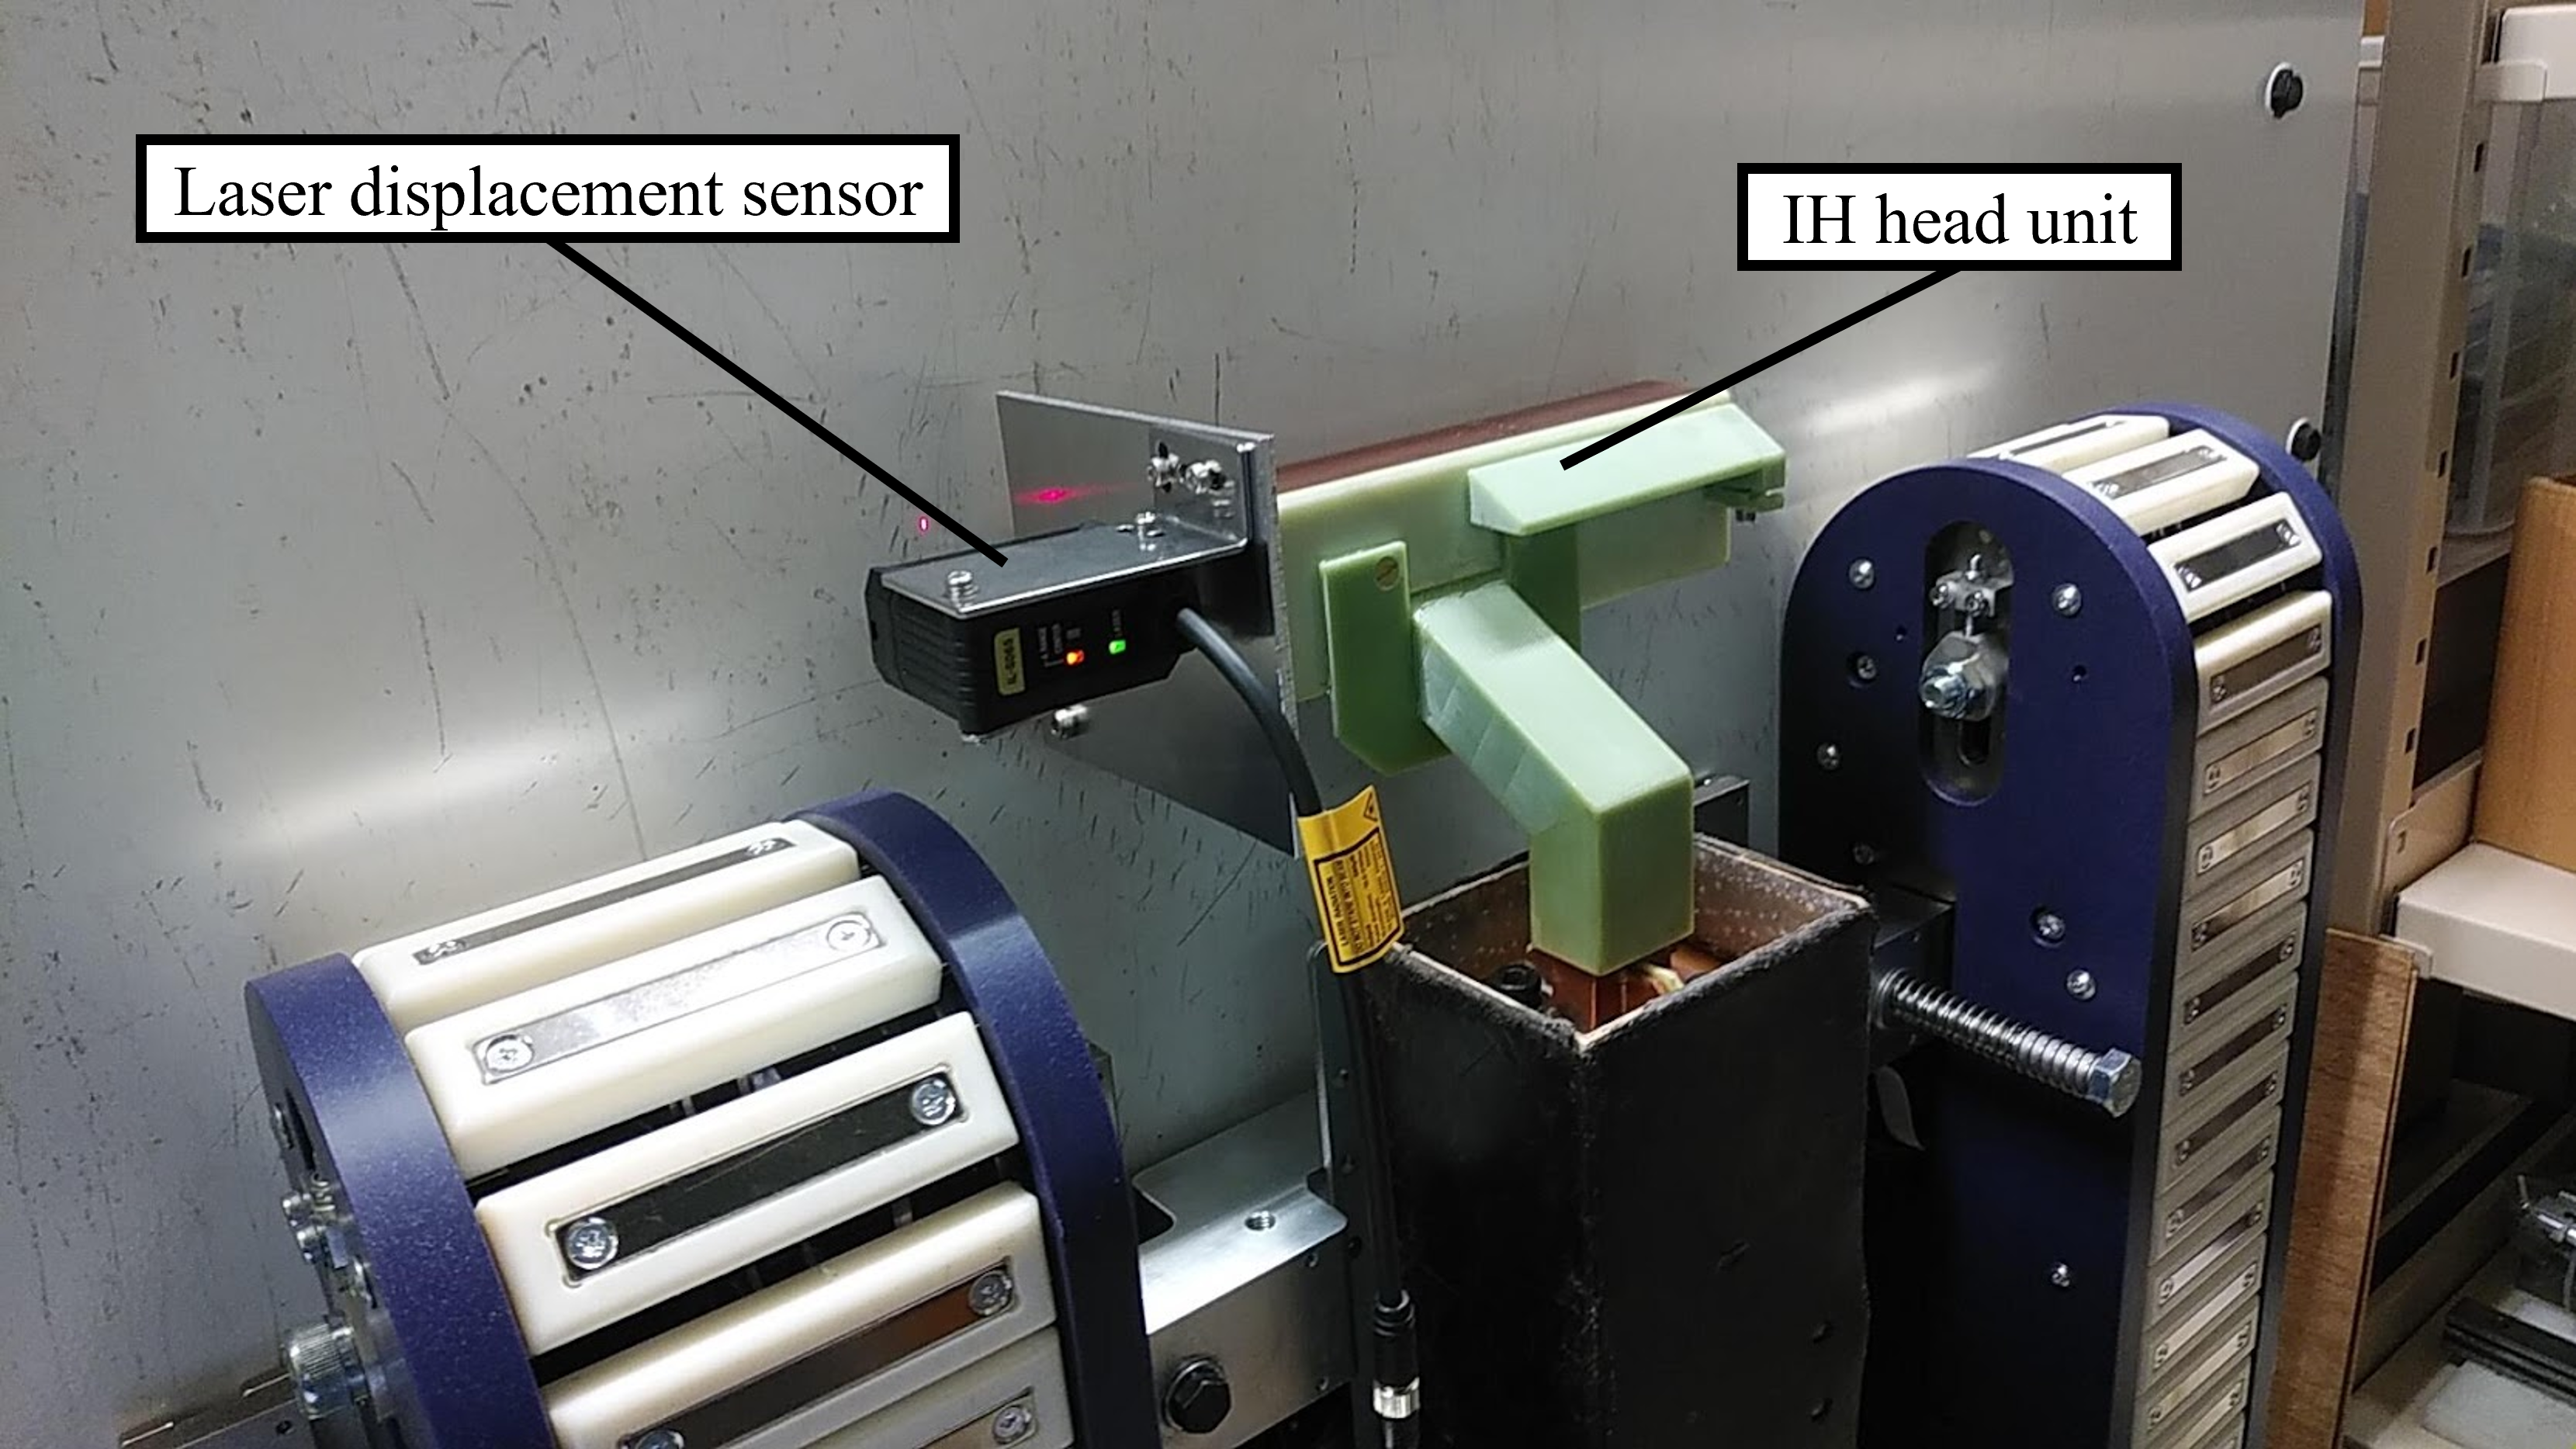
\includegraphics[width=0.8\textwidth]{full/displacement_full_pic.png}
  \caption{Full scale robot with laser displacement sensor}
  \label{full laser}
\end{figure}

\begin{figure}[H]
  \begin{minipage}{0.57\hsize}
    \centering
    \includegraphics[height=45mm]{displacement.png}
    \caption{Displacement of half-scale robot}
    \label{dis_half}
  \end{minipage}
  \begin{minipage}{0.43\hsize}
    \centering
    \includegraphics[height=45mm]{full/displacement_full}
    \caption{Displacement of full-scale robot}
    \label{dis_full}
  \end{minipage}
\end{figure}	

\begin{table}[H]
  \label{compare}
  \centering
  \caption{Maximum displacement during wall running}
  \begin{tabular}{c|cc}
  body   magnet    & without      & with         \\ \hline
  half-scale robot & 0.42{[}mm{]} & 0.16{[}mm{]} \\
  full-scale robot & 0.19{[}mm{]} & 0.20{[}mm{]}
  \end{tabular}
\end{table}


\newpage
\section{壁面への取り付け・取り外し機構の検討}
機体全体の磁石の吸着力は4000[N]以上となるため安全に壁面への取り付け及び取り外しを行うためには専用の機構が必要であると考えた. 機体に設けた雌ねじに対し雄ネジを取り付けこれを突っ張ることで安全に壁面への取り付及び取り外しを行うことができると考えた. 安定して突っ張ることができるように雄ネジの先端にはボールジョイントを持つスイベルナットを取り付ける設計とした. 

以下の式(\cite{nezi}より導出)より機体を取り外す際に必要なトルクを概算した. 
\begin{equation}
  t = F \frac{d}{2} \times \frac{p + \mu \pi d}{\pi d - \mu p}
\end{equation}

$F = 5000[N], d = 10[mm], p = 1[mm], \mu = 0.5$のときトルクは$t = 13.5[Nm]$となった. 一般的な工具で取り外すことが可能であることを確認した. 

\begin{figure}[H]
  \centering
  \includegraphics[width=0.7\textwidth]{full/bolt.png}
  \caption{Diagram of bolts for mounting and dismounting}
  \label{bolt}
\end{figure}

塗膜剥離試験において取り付け・取り外しを行った際, IHヘッドを取り外した状態において機体を最下部に接触させ上部2個のボルトを交互に回すことにより機体の上部が浮き上がり容易に取り外しを行うことができた. 
\begin{figure}[H]
  \centering
  \includegraphics[width=0.7\textwidth]{full/remove_robot.png}
  \caption{Dismounting the robot}
  \label{dismounting}
\end{figure}  

\newpage
\section{中央フレームの設計}

前節で述べた機体の取り付け及び取り外しに使用すねじの雌ねじは中央フレームに設けてある. そのため, 中央フレームは取り付け及び取り外しの際に大きい力を受ける. そのため, Autodesk Inventor Nastranを用い, 解析を行い試行錯誤的に設計を行った. 本節ではその解析条件の設定や解析結果について述べる. 

\begin{figure}[H]
  \centering
  \includegraphics[width=0.5\textwidth]{center/center-flame_3d.png}
  \caption{Center flame}
  \label{center_flame}
\end{figure}

\subsection{小型モデルによる検証}

検討した解析条件が適切であるか検証するため, 小型モデルで解析と実験を行った. 中央フレームと機体の磁石を模した, ジュラルミン(A2017)製の部材に磁石を取り付けたものを製作した. 磁石の鋼板の接地面の端を基準としたモーメントを考え, ボルトが磁石を引きはがす直前にボルトが出すモーメントと磁石によるモーメントがつい合うと考えた. その時のボルトの力が中央フレームにかかる最大に力と考えた. 式\ref{eq_of_center-mini}より磁石を引きはがす時にボルトにかかる最大の力が求められる.

\begin{equation}
\label{eq_of_center-mini}
  F_{s} = \frac{F_{m1}a + F_{m2}c}{b}
\end{equation}

\begin{figure}[H]
  \centering
  \includegraphics[width=0.6\textwidth]{center/moment_mini.png}
  \caption{Moment diagram of small model}
  \label{}
\end{figure}

\newpage

以上について, Inventor Nastranによる解析及び実験を行った. 磁石を取り付ける両端部の下側の線をピン拘束し, ボルトを設ける雌ねじ部に荷重をかけた. また, 実際に製作した模型の実験においてボルトにトルクをかけ, 磁石が剥離する直前の最大の変位を計測した. この変位が解析の最大変位と概ね一致した. これにより, 解析条件に妥当性があると考えた.

\begin{figure}[H]
  \begin{minipage}{0.5\hsize}
    \centering
    \includegraphics[width=1\textwidth]{center/model_fem.png} 
    \caption{Analysis of small models}
    \label{}
  \end{minipage}
  \begin{minipage}{0.5\hsize}
    \centering
    \includegraphics[width=1\textwidth]{center/model_pic.jpg}
    \caption{Testing with small models}
    \label{}
  \end{minipage}
\end{figure}	

\subsection{フルスケール機体設計のための解析}

実際の中央フレームについて解析を行うために前項と同様にボルトにかかる力を求めた. 実際の機体においてボルトは機体の四隅の内側に位置する. そのため, クローラの進行方向のモーメント(図\ref{moment_full_side_zu}, 式\ref{moment_full_side})も考慮する必要がある. 今回は簡単のため, ボルト側のクローラユニットのみ進行方向のモーメントを計算に含めた(式\ref{moment_full}).
$F_{m2}$に式\ref{eq_of_absorb}より得られた吸着力を代入し, $F_{m1}$に図\ref{yoke-graph-full}で得られた吸着力をフレーム磁石ユニットに用いた個数(10個)分乗じた値を代入した.

\begin{equation}
  \label{moment_full_side}
  F'= F'_m \frac{B}{A}
\end{equation}

\begin{equation}
  \label{moment_full}
  F = \frac{F_{m1}b+F_{m2}(c-a)+\frac{B}{A}\{F_{m1}f+F_{m2}(d+g)\}}{e}
\end{equation}

\begin{figure}[H]
  \centering
  \includegraphics[bb = 0 0 525 334, width=0.25\textwidth]{center/moment_side.png}
  \caption{Moment diagram of full scale robot (size view)}
  \label{moment_full_side_zu}
\end{figure}	

\begin{figure}[H]
  \centering
  \includegraphics[width=0.60\textwidth]{center/moment_front.png}
  \caption{Moment diagram of full scale robot (front view)}
  \label{moemnt_full_zu}
\end{figure}


式\ref{moment_full}で得られた値を用い解析を行った. 中央フレームの解析においては, 中央フレームとクローラユニットを固定する外側のボルト穴を図\ref{full-FEM}におけるZ軸周りのピン拘束とした. 結果, 降伏点の安全率約1.36, 最大変位約0.3[mm]となる寸法を採用した. 実際の機体においては, クローラユニットとの結合により剛性が増すため, より強度は高くなると考えらえる. 

\begin{figure}[H]
  \centering
  \includegraphics[width=1\textwidth]{center/center-FEM.png}
  \caption{Analysis of small models}
  \label{full-FEM}
\end{figure}

\newpage
\section{段差の乗り越え実験}

塗膜剥離後の面と未剥離の面の段差, 塗装の凸凹などの段差を踏破する必要がある. 本節では, 直進時と旋回時における段差乗り越えの実験について述べる.

\subsection{直進時の段差乗り越え実験}

段差は, 約150[mm]角, 厚さ2[mm]の樹脂版を厚さ0.16[mm]の両面テープで実験用鋼板に貼り付けて設置した. 左右両側のクローラユニットの同時乗り越え(図\ref{env of step simu})と, 片側のクローラユニットの乗り越え(図\ref{env of step one})についてそれぞれ上昇及び下降における段差乗り越えの実験を行った. 結果, 問題なく段差踏破が行えることを確認した. 

\begin{figure}[H]
  \begin{minipage}{0.5\hsize}
    \centering
    \includegraphics[width=0.9\textwidth]{full/step1.png}
    \caption{Simultaneous step over test}
    \label{env of step simu}
  \end{minipage}
  \begin{minipage}{0.5\hsize}
    \centering
    \includegraphics[width=0.9\textwidth]{full/step2.png}
    \caption{One-side step over test}
    \label{env of step one}
  \end{minipage}
\end{figure}	

\begin{figure}[H]
  \centering
  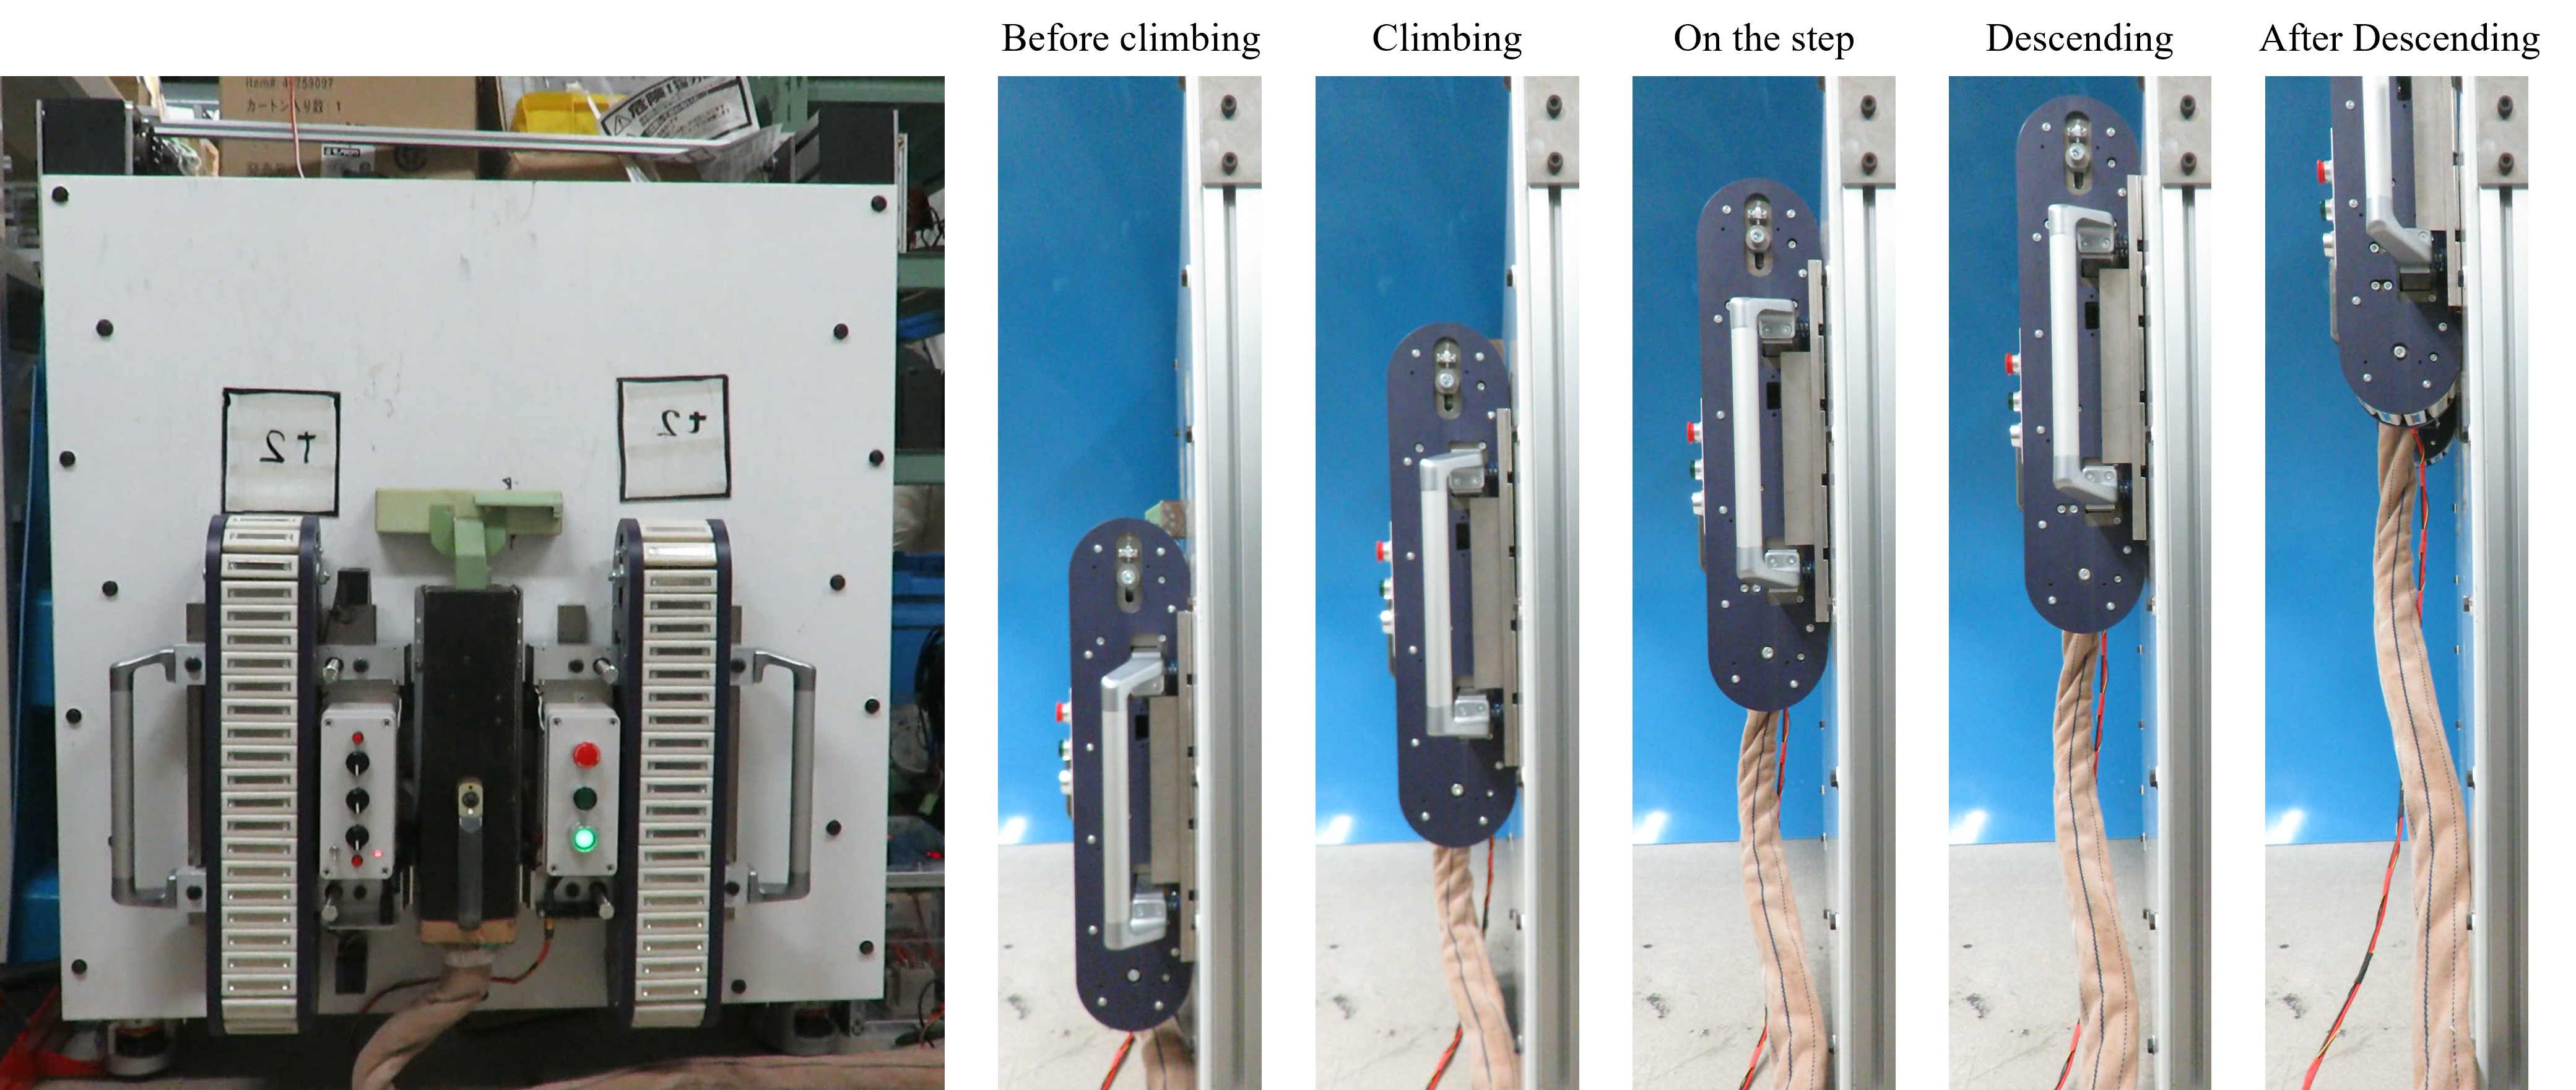
\includegraphics[width=1\textwidth]{full/step_side.png}
  \caption{Side view of step over test}
  \label{side view step}
\end{figure}

\newpage
\subsection{旋回時の段差乗り越え試験}

フルスケール機体は履板の接地面全周囲にフィレットを設けることで超信地旋回時もある程度の段差踏破能力を持たせた. 
旋回時の乗り越え可能段差高さは壁面とレールの部材及びフレーム磁石距離に依存する. 壁面とレールの部材の距離が1[mm]であるため(図\ref{step_cad}), 壁面とフレーム磁石の距離を1[mm]以上に調整してあるとき, 1[mm]未満の段差であれば踏破可能と考えた. そこで, 約30[mm]角, 厚さ0.7[mm]の樹脂板を0.16[mm]の両面テープで複数個無秩序に実験用鋼板に貼り付けて超新地旋回を行う実験を行った(図\ref{random step test}). 結果, 問題なく超新地旋回を行うことができた. 

\begin{figure}[H]
  \centering
  \includegraphics[width=1\textwidth]{full/side_step.png}
  \caption{Distance between rail member and wall surface}
  \label{step_cad}
\end{figure}

\begin{figure}[H]
  \centering
  \includegraphics[width=0.6\textwidth]{full/step3.png}
  \caption{Step over test in turning}
  \label{random step test}
\end{figure}

%\section{製作}

\newpage
\section{塗膜剥離試験}
実際の鋼橋に使用されるのと同様の試験桁を用いた, 塗膜剥離試験を行った.
%試験環境の詳細は\textgt{付録F}の試行案に掲載されている.
試験環境の詳細は\textgt{付録F}に掲載した.
図\ref{env_of_remove}に実験環境の写真を示す. 

\begin{figure}[H]
  \centering
  \includegraphics[width=1\textwidth]{const/env_of_test.JPG}
  \caption{Enviroment of removing test}
  \label{env_of_remove}
\end{figure}

\newpage

\subsection{垂直加熱試験}
縦方向に移動し過熱を行う垂直加熱試験を行った. その様子を図\ref{vertical}に示す. 過熱され鏡面破壊を起こした塗膜がしわになっている様子が確認できる. 

\begin{figure}[H]
  \centering
  \includegraphics[width=0.5\textwidth]{const/vertical-test.png}
  \caption{Vertical heating test}
  \label{vertical}
\end{figure}

\newpage

\subsection{塗膜の除去作業}
一度過熱し界面破壊を起こした塗膜の除去作業はスクレーパーを用いて容易に除去することができる. このため, 除去作業は従来通り作業員が行うことを想定している. 過熱後に, 筆者がその作業の体験も兼ねてを除去作業を行った(図\ref{remove}). 今回の試験でもスクレーパーを用いて容易に除去することができた.

\begin{figure}[H]
  \centering
  \includegraphics[width=1\textwidth]{const/vh.png}
  \caption{Removing paint film}
  \label{remove}
\end{figure}  

\subsection{自律移動試験}
自律移動試験を行った. 姿勢制御は1/2スケール機体(\ref{1/2auto})と同様のIMUとアルゴリズムを用いた.
IHヘッドの電源を入れたところ, 回路が誤動作を起こした. IHヘッドの高周波ノイズが機体の回路の動作に影響を与えたと考えられる. 
そのため, 過熱は行わず自律移動の試験のみを行たった.

\begin{figure}[H]
  \centering
  \includegraphics[height=0.9\textheight]{const/auto-full-1.png }
  \caption{Auto moving test 1}
  \label{auto-full}
\end{figure}

\begin{figure}[H]
  \centering
  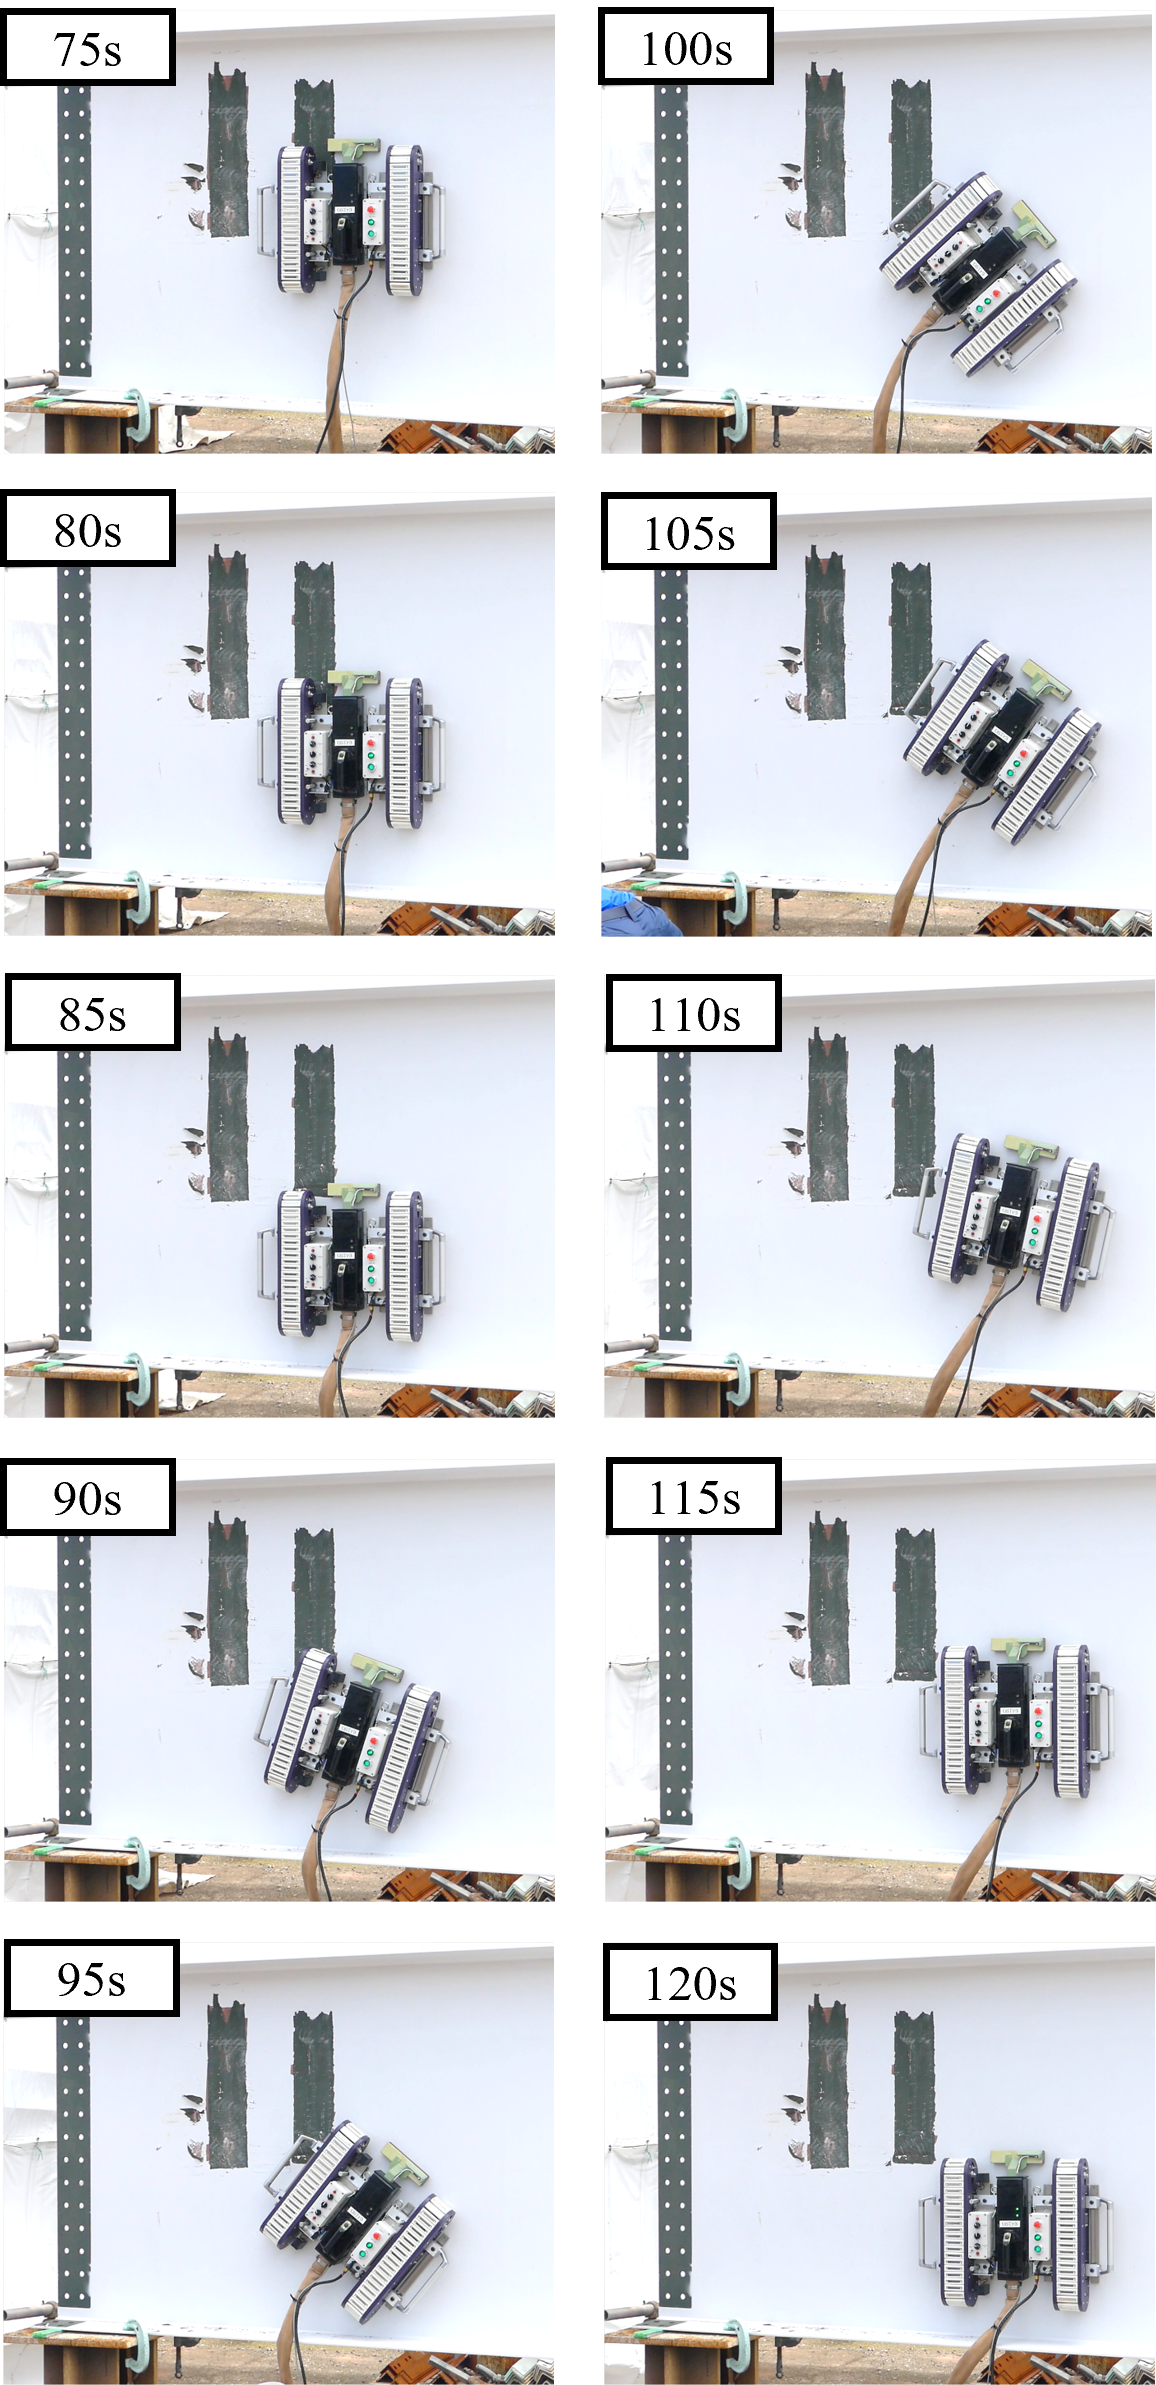
\includegraphics[height=0.9\textheight]{const/auto-full-2.png}
  \caption{Auto moving test 2}
  \label{auto-full-2}
\end{figure}
\newpage

\subsection{左端部及び下端部加熱試験}
現状の自律動作のみでは, IHヘッド加熱部の位置と機体のサイズにより, 左右と下の端部の過熱を行うことができない. そこで, ゲームパッドを用いた手動操作にて左端部及び下端部の過熱を行った.図\ref{horizonal}に示すように機体を90度旋回させ, 水平方向に移動することで左端部の過熱を行うことができる. また, 図\ref{turn}のように180度旋回させ機体を上下反転させることで下端部の過熱が可能になる. 図\ref{lower}に下端部を起点とする垂直加熱試験の様子を示す.

\begin{figure}[H]
  \begin{minipage}{0.5\hsize}
    \centering
    \includegraphics[width=0.9\textwidth]{const/horizonal-test.png}
    \caption{Horizonal heating test}
    \label{horizonal}
  \end{minipage}
  \begin{minipage}{0.5\hsize}
    \centering
    \includegraphics[width=0.9\textwidth]{const/turn.png}
    \caption{Turning}
    \label{turn}
  \end{minipage}
\end{figure}	

\begin{figure}[H]
  \centering
  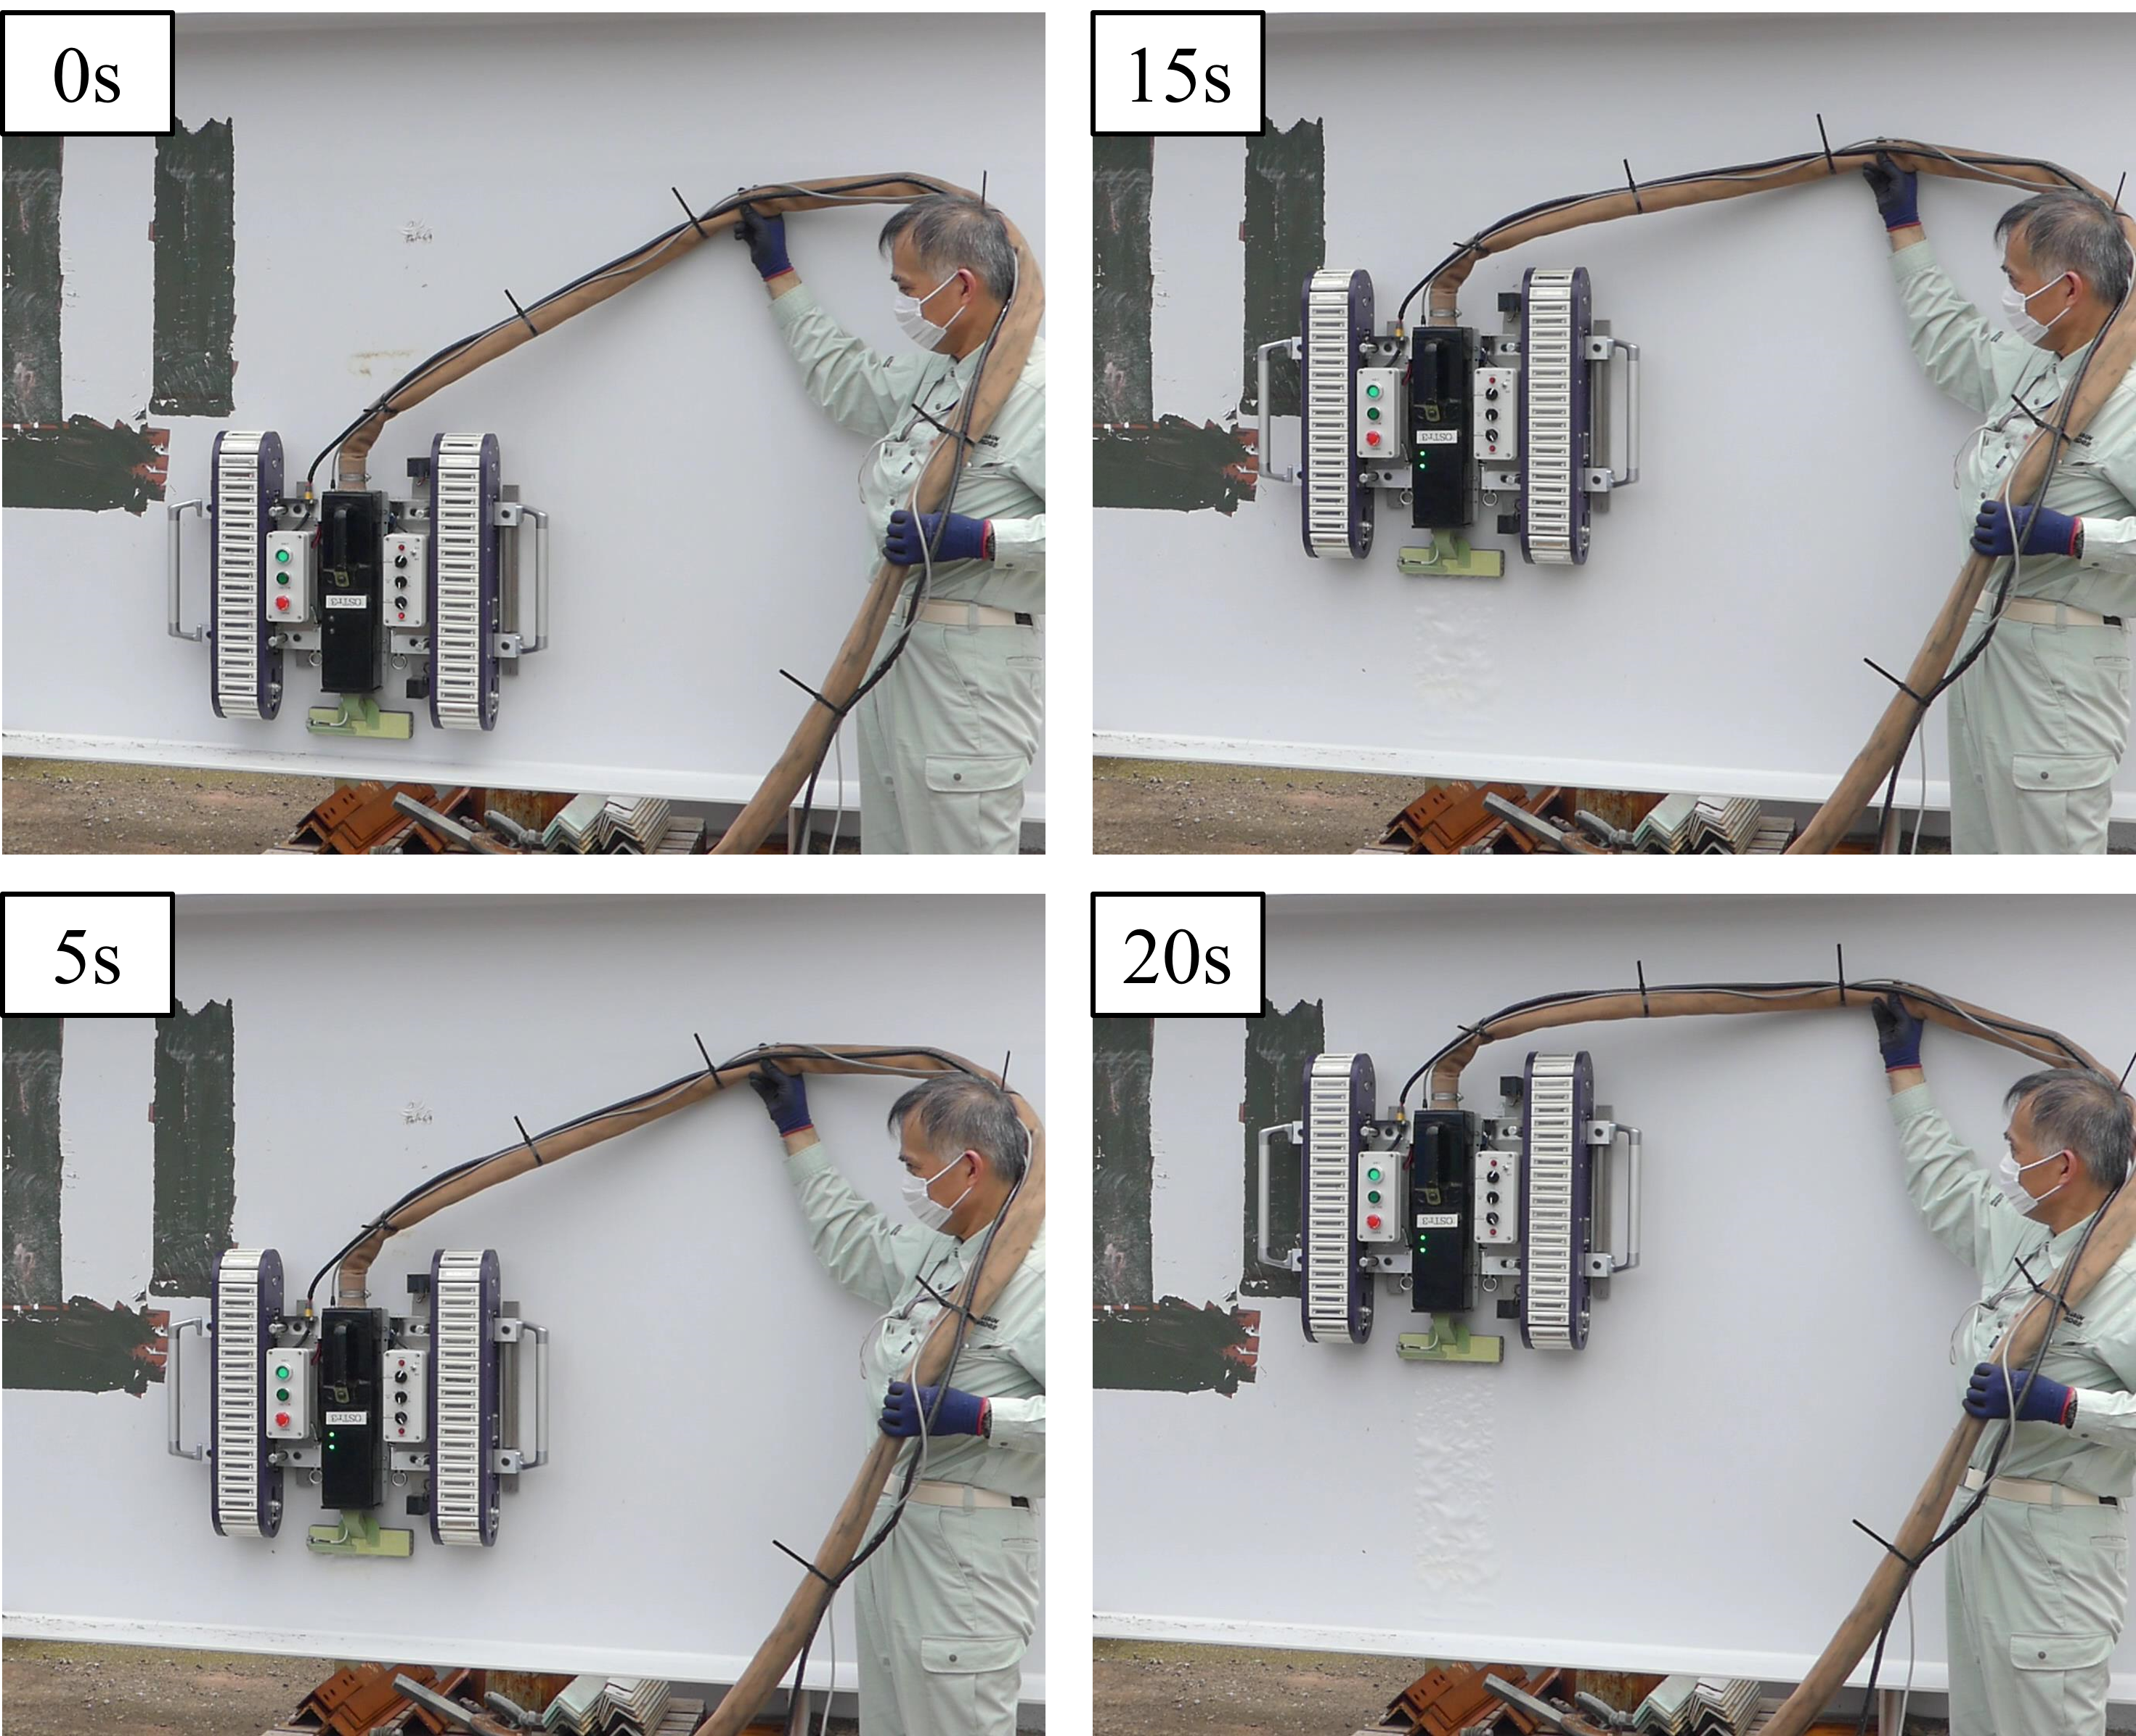
\includegraphics[width=1\textwidth]{const/lower.png}
  \caption{Lower side heating test}
  \label{lower}
\end{figure}

\newpage

\subsection{壁面の熱による履板及び磁石の影響調査}
\label{netu}
赤外線サーモグラフィにより試験中の鋼板や機体の温度を計測した. 試験は真夏日の昼間, 直射日光下で行われたため, 壁面の温度はその影響も受けていると考えられる. 本項ではサーモグラフィを踏まえ, 考えられる熱による履板及び磁石の影響について述べる.

\subsubsection{加熱時における履板への影響}
過熱試験時のサーモグラフィを以下に示す. 上部は垂直過熱試験を行った際の熱が残っているため比較的高温となっているが, IHヘッドによる過熱は局所的なものであることが分かる. 

\begin{figure}[H]
  \centering
  \includegraphics[width=0.3\textwidth]{thermo/1st}
  \caption{Thermography of heating test}
  \label{heat1}
\end{figure}  

\subsubsection{加熱直後の加熱部の通過による履板への影響}
自動垂直加熱において, 次の列に移動する際に直前の過熱部を通過する必要がある. この時の熱による履板や磁石への影響について述べる. 直前に加熱した箇所を通過した時のサーモグラフィを以下に示す. 通過後(図\ref{after_pass})左のクローラユニット履帯が, 1部100[\si{\degreeCelsius}]以上まで加熱されていることが分かる. 

\begin{figure}[H]
  \begin{minipage}{0.5\hsize}
    \centering
    \includegraphics[width=0.6\textwidth]{thermo/2nd}
    \caption{Thermography of robot passing through heated spot 1}
    \label{before_pass}
  \end{minipage}
  \begin{minipage}{0.5\hsize}
    \centering
    \includegraphics[width=0.6\textwidth]{thermo/3rd}
    \caption{Thermography of robot passing through heated spot 2}
    \label{after_pass}
  \end{minipage}
\end{figure}

\subsubsection{磁石の熱に対する影響}
磁石は, 温度が高いほど吸着力が低下する. 温度と吸着力の関係をフルスケール機体に使用した磁石の販売元である株式会社マグファインの磁気計算器\cite{magfine_cal}を用いて調べた. 2つの取付穴は設定不能なため計算に含まれていない. これにより得られた鉄板とのギャップ1[mm]時の温度と吸着力のグラフを以下に示す. フルスケール機体に用いたネオジム35のほか, より耐熱温度の高いネオジム35UH, サマリウムコバルトYXG28についても調べた. 磁石は耐熱温度未満であれば冷やすことで吸着力が回復するが, 超えると不可逆変化となり吸着力は回復しない\cite{magfine_faq}.

図\ref{heat1}の下側の温度は約60[\si{\degreeCelsius}]となり20[\si{\degreeCelsius}]と比較すると, 吸着力は約86[\%]まで低下しいてることが分かる.
さらに, 図\ref{after_pass}の際, 磁石の吸着力が不可逆変化の領域まで低下していることが考えられる. 
今回は機体の動作に影響はなかったが, 塗膜厚や摩擦係数などの条件により影響が出る可能性があるため, ネオジム35UHなどの耐熱性の高い磁石を使用する必要があると考えた. 

\begin{table}[H]
  \centering
  \caption{Heat resistance temperature of magnet}
  \begin{tabular}{r|c}
  磁石材料           & 耐熱温度{[}\si{\degreeCelsius}{]} \\ \hline
  ネオジム35         & 80          \\
  ネオジム35UH       & 180         \\
  サマリウムコバルトYXG28 & 300        
  \end{tabular}
\end{table}

\begin{figure}[H]
  \centering
  \includegraphics[width=0.9\textwidth]{thermo/temp2.png}
  \caption{Relationship between temperature and adsorption force when 1[mm] gap with iron}
  \label{temp}
\end{figure}

\subsection{履板材料への影響}
履板に使用しているABSは最大連続使用温度が50[\si{\degreeCelsius}]であるため\cite{zyusi}, 長期的な運用により変形等の影響がでる可能性がある. そのためより適した履板材料として表\ref{selection}, 図\ref{track-shoe_friction}に示すようにより耐熱性が高く同等の動摩擦係数を持つPC(ポリカーボネート)などが考えられる. 

\newpage

\subsection{メカナム機体との比較}

塗膜剥離試験は, 米田研究室の綱川が製作したメカナムホイール機体\cite{meca-s}についても行った. メカナムホイール機体は全方位移動が行えるため, 本研究のクローラ機体と比較すると, より短時間で次の列の塗装に移行できる. しかし, 水平加熱試験においては水平を維持できずに徐々に下に下がる現象が確認された(図\ref{mecanum}). また, 界面破壊した塗膜などの段差の踏破性能もクローラ機体と比較して低かった.
 コストの観点においては, メカナム機体がモータ数が4つに対しクローラ機体が2つである点ではクローラ機体が有利である. 一方その他の部品においては, 磁気クローラにおける履板やレールなどの専用部品を数多く用いるクローラ機体に対して, 既存のメカナムホイールを用いるメカナム機体のほうが有利であると考えられる. クローラ機体の製作コスト参考のため, 外注部品の見積書を\textgt{付録E}に掲載した.
 今回はこれらの違いを総合的に判断し, 水平方向の剥離や段差における安定性の高いクローラ機体の開発が継続されることとなった.

\begin{figure}[H]
  \centering
  \includegraphics[width=1\textwidth]{const/mecanum.png}
  \caption{Side heating test of mecanum wheel robot}
  \label{mecanum}
\end{figure}

\begin{table}[H]
  \centering
  \caption{Comparison of mechanum and crawler robots}
  \begin{tabular}{r|cc}
          & メカナム機体  & クローラ機体 \\ \hline
  全方位移動   & 〇       & ×      \\
  段差踏破    & △       & 〇      \\
  水平方向の剥離 & △       & 〇      \\
  モータ数    & 4       & 2      \\
  走行部の部品  & 既製品が利用可 & 専用部品多数
  \end{tabular}
\end{table}

\begin{comment}
\section{動摩擦係数の変化要因の調査}
\subsection{圧力}
\subsection{速度}
\subsection{温度及び湿度}  
\end{comment}
